%%%%%%%%%%%%%%%%%%%%%%%%%%%%%%%%%%%%%%%%%%%%%%%%%%%%%%%%%%%%%%%%%%%%%%%%%%%%%%%%
% ARTIGO CIENTÍFICO — modelo abnTeX2 (formato "article")
% Conformidade com ABNT: NBR 14724, NBR 6023, NBR 6024, NBR 6028, NBR 10520.
%
% Como compilar (Overleaf): Menu > Compiler = pdfLaTeX. A sequência é
%   pdfLaTeX -> BibTeX -> pdfLaTeX -> pdfLaTeX  (o Overleaf faz isso ao
%   clicar em "Recompile"; se as citações saírem como [?], recompile de novo).
%
% Edite APENAS o conteúdo. Os arquivos abntex2.cls, abntex2cite.sty e
% abntex2-alf.bst NÃO precisam ser editados.
%%%%%%%%%%%%%%%%%%%%%%%%%%%%%%%%%%%%%%%%%%%%%%%%%%%%%%%%%%%%%%%%%%%%%%%%%%%%%%%%

\documentclass[
	article,			% formato de artigo (seções em vez de capítulos)
	11pt,				% tamanho da fonte
	oneside,			% impressão só frente
	a4paper,			% tamanho do papel
	% -- opções do babel --
	english,			% idioma adicional (resumo em inglês)
	brazilian,			% idioma principal do documento
	sumario=tradicional
	]{abntex2}

% ---------------------------------------------------------------------------
% PACOTES
% ---------------------------------------------------------------------------
\usepackage[utf8]{inputenc}		% acentuação (UTF-8)
\usepackage[T1]{fontenc}		% codificação das fontes
\usepackage{lmodern}			% fonte Latin Modern
\usepackage{indentfirst}		% indenta o primeiro parágrafo de cada seção
\usepackage{graphicx}			% figuras
\usepackage{xcolor}			% cores
\usepackage{microtype}			% melhorias de justificação
\usepackage{amsmath,amssymb}		% matemática
\usepackage{booktabs}			% linhas de tabela mais elegantes
\usepackage{array}
\usepackage{multirow}
\usepackage{longtable}
\usepackage{listings}			% blocos de código
\usepackage{url}
\usepackage{tikz}			% diagramas / fluxogramas
\usetikzlibrary{shapes.geometric,arrows.meta,positioning,fit,backgrounds}
\usepackage{float}			% posicionamento [H] para os fluxogramas
% Float "Quadro" (ABNT: conteúdo textual/esquemático, distinto de "Tabela").
% Estilo próprio: legenda no topo e separador em travessão (como Figuras/Tabelas).
\makeatletter
\newcommand\floatc@abnttop[2]{\setbox\@tempboxa\hbox{{\@fs@cfont #1 \textendash\ }#2}%
	\ifdim\wd\@tempboxa>\hsize {\@fs@cfont #1 \textendash\ }#2\par
	\else\hbox to\hsize{\hfil\box\@tempboxa\hfil}\fi}
\newcommand\fs@abnttop{\fs@plaintop\let\@fs@capt\floatc@abnttop}
\makeatother
\floatstyle{abnttop}
\newfloat{quadro}{htbp}{loq}
\floatname{quadro}{Quadro}
\floatstyle{plain}

% ---- Citações e referências padrão ABNT (autor-data) ----
\usepackage{hyperref}
\usepackage[brazilian,hyperpageref]{backref}
\usepackage[alf,abnt-emphasize=bf,abnt-etal-cite=3,abnt-etal-list=0]{abntex2cite}

% Configuração do backref (mostra em que página cada referência foi citada)
\renewcommand{\backrefpagesname}{Citado na(s) página(s):~}
\renewcommand{\backref}{}
\renewcommand*{\backrefalt}[4]{%
	\ifcase #3 %
		(Nenhuma citação no texto.)%
	\or
		(Citado na página #2.)%
	\else
		(Citado #3 vezes nas páginas #2.)%
	\fi}

% Cores dos links (discretas)
\definecolor{azulref}{RGB}{0,80,160}
\hypersetup{
	colorlinks=true,
	linkcolor=black,
	citecolor=azulref,
	urlcolor=azulref,
	pdftitle={Diagnostico de defeitos de impressao em etiquetas de codigos de barras},
	pdfauthor={Saymon Coppi de Oliveira Silva},
	pdfsubject={Visao computacional e orquestracao multiagente},
	pdfkeywords={codigo de barras, visao computacional, ADK, defeitos de impressao}
}

% ---- Estilo dos blocos de código ----
\definecolor{codebg}{gray}{0.96}
\definecolor{codecomment}{RGB}{0,120,0}
\definecolor{codestring}{RGB}{160,0,120}
\definecolor{codekw}{RGB}{0,0,180}
\lstset{
	basicstyle=\ttfamily\footnotesize,
	backgroundcolor=\color{codebg},
	keywordstyle=\color{codekw}\bfseries,
	commentstyle=\color{codecomment}\itshape,
	stringstyle=\color{codestring},
	numbers=left, numberstyle=\tiny\color{gray}, numbersep=7pt,
	breaklines=true, showstringspaces=false, frame=single,
	rulecolor=\color{gray!50}, captionpos=b, tabsize=2, columns=fullflexible,
	literate=%
		{á}{{\'a}}1 {é}{{\'e}}1 {í}{{\'i}}1 {ó}{{\'o}}1 {ú}{{\'u}}1
		{Á}{{\'A}}1 {É}{{\'E}}1 {Í}{{\'I}}1 {Ó}{{\'O}}1 {Ú}{{\'U}}1
		{à}{{\`a}}1 {â}{{\^a}}1 {ê}{{\^e}}1 {ô}{{\^o}}1 {ç}{{\c c}}1
		{ã}{{\~a}}1 {õ}{{\~o}}1 {Ç}{{\c C}}1 {Ã}{{\~A}}1 {Õ}{{\~O}}1
}

% ---------------------------------------------------------------------------
% DADOS DO TRABALHO  >>> EDITE AQUI <<<
% ---------------------------------------------------------------------------
\titulo{Diagnóstico de defeitos de impressão em etiquetas de códigos de barras: uma abordagem por visão computacional e orquestração multiagente}

% Título em inglês (obrigatório no modelo de artigo abnTeX2: é impresso abaixo do título)
\tituloestrangeiro{Diagnosis of printing defects in barcode labels: an approach based on computer vision and multi-agent orchestration}

\autor{Saymon Coppi de Oliveira Silva\thanks{Universidade Federal de São Paulo
	(Unifesp), Instituto de Ciência e Tecnologia. Programa de Pós-Graduação em
	Ciência da Computação. Disciplina: Visão Computacional (cód.~2587), Prof. Dr.
	Fabio Augusto Menocci Cappabianco. E-mail: \texttt{saymoncoppi@gmail.com}.}}

\local{São José dos Campos}
\data{2026}

% Logo da instituição no topo da 1ª página (antes do título) — hook do memoir
\renewcommand{\maketitlehooka}{%
	\begin{center}
		
\includegraphics[width=5cm]{figuras/unifesp.png}
	\end{center}
	\vspace{0.4cm}%
}

% ===========================================================================
\begin{document}

\selectlanguage{brazilian}
\frenchspacing

% Título, autor e nota de rodapé de filiação
\maketitle

% ---------------------------------------------------------------------------
% RESUMO (português) — NBR 6028: 150 a 500 palavras, parágrafo único,
% linguagem impessoal, sem citações.
% ---------------------------------------------------------------------------
\begin{resumoumacoluna}
A leitura confiável de códigos de barras depende da qualidade de impressão das
etiquetas, avaliada por normas como a ISO/IEC 15416; contudo, os verificadores
certificados são caros e reportam apenas uma nota, sem indicar a causa física
do defeito nem a ação corretiva. Este trabalho propõe e desenvolve um sistema de
baixo custo que, a partir de uma imagem capturada por um dispositivo comum,
detecta defeitos típicos de impressão em etiquetas de códigos de barras e sugere
sua causa provável. A solução combina visão computacional --- uma rede neural
convolucional com \textit{backbone} leve, treinada por transferência de
aprendizado --- e orquestração multiagente com o \textit{Agent Development Kit}
(ADK), decompondo a tarefa em leitura/decodificação, estimativa de indicadores de
qualidade, detecção de defeitos físicos e diagnóstico de causa-raiz fundamentado
na documentação técnica do fabricante --- estágio que, além dos resultados
anteriores, inspeciona a própria imagem (multimodal) e pode arbitrar a
classificação da rede nos pares visualmente confundíveis. O sistema é exposto por uma \textit{API}
única, consumida por uma interface web responsiva, acessível de qualquer
dispositivo com navegador --- computador, \textit{notebook}, \textit{tablet} ou
celular ---, independentemente do sistema operacional. A avaliação emprega um
conjunto de dados híbrido --- imagens reais de captura e defeitos de impressão
gerados sinteticamente de forma controlada e reprodutível --- e, para a
classificação de defeitos, compara a CNN adotada (MobileNetV3-Small) a
arquiteturas de referência (ResNet18 e EfficientNet-B0) sob protocolo idêntico,
com validação cruzada estratificada e teste de significância estatística. Os
resultados demonstram a viabilidade de um apoio à decisão que vai além da nota,
indicando causa provável e correção sugerida.

\noindent
\textbf{Palavras-chave}: código de barras; qualidade de impressão; visão
computacional; aprendizado profundo; sistemas multiagentes.
\end{resumoumacoluna}

% ---------------------------------------------------------------------------
% ABSTRACT (inglês)
% ---------------------------------------------------------------------------
\begin{resumoumacoluna}[Abstract]
\begin{otherlanguage*}{english}
Reliable barcode reading depends on the print quality of the labels, which is
assessed by standards such as ISO/IEC 15416; however, certified verifiers are
expensive and report only a grade, without indicating the physical cause of the
defect or the corrective action. This work proposes and develops a low-cost
system that, from an image captured by an ordinary device, detects typical
printing defects in barcode labels and suggests their probable cause. The
solution combines computer vision --- a convolutional neural network with a
lightweight backbone, trained by transfer learning --- and multi-agent
orchestration with the Agent Development Kit (ADK), decomposing the task into
reading/decoding, quality-indicator estimation, physical-defect detection and
root-cause diagnosis grounded in the manufacturer's technical documentation --- a
stage that, beyond the previous results, also inspects the image itself
(multimodal) and can arbitrate the network's classification for visually
confusable pairs. The
system is exposed through a single API, consumed by a responsive web interface
accessible from any device with a browser --- desktop, notebook, tablet or
smartphone ---, regardless of the operating system. The evaluation uses a hybrid
dataset --- real capture images and printing defects generated synthetically in a
controlled and reproducible way --- and, for defect classification, compares the
adopted CNN (MobileNetV3-Small) against reference architectures (ResNet18 and
EfficientNet-B0) under an identical protocol, with stratified cross-validation and
a statistical significance test. The results demonstrate the feasibility of a
decision-support tool that goes beyond the grade, pointing to a probable cause and
a suggested correction.

\noindent
\textbf{Keywords}: barcode; print quality; computer vision; deep learning;
multi-agent systems.
\end{otherlanguage*}
\end{resumoumacoluna}

% Sumário (opcional em artigos; comente as duas linhas abaixo se não quiser)
\tableofcontents*
\newpage

% ===========================================================================
\textual
% ===========================================================================

% ---------------------------------------------------------------------------
\section{Introdução}
% ---------------------------------------------------------------------------

\subsection{Contextualização}

Códigos de barras são a espinha dorsal da identificação automática de itens em
varejo, logística, saúde e manufatura. Uma etiqueta é lida dezenas de vezes ao
longo da cadeia --- na expedição, no transporte, no recebimento e no ponto de
venda --- e cada leitura pressupõe que a impressão preserve as proporções de
barras e espaços dentro de tolerâncias estreitas. Quando a impressão degrada, o
custo não é apenas uma releitura: há reprocessamento manual, atraso operacional,
devolução de cargas e, em setores regulados, não conformidade.

Por essa criticidade, a qualidade de impressão é normatizada. A norma ISO/IEC
15416 define, para símbolos lineares (1D), um conjunto de parâmetros objetivos
derivados do \textit{perfil de refletância de varredura} --- entre eles contraste
do símbolo, modulação, decodificabilidade e defeitos --- que são convertidos em
notas de A a F \cite{iso15416}. Para símbolos bidimensionais (2D), a ISO/IEC
15415 cumpre papel análogo \cite{iso15415}, e a conformidade dos aparelhos
verificadores é regida pela ISO/IEC 15426 \cite{iso15426}. Na prática industrial,
essa avaliação é feita por \textit{verificadores ópticos} dedicados, equipamentos
calibrados e de custo elevado.

Paralelamente, no chão de fábrica, os defeitos de impressão têm origem física bem
conhecida e documentada pelos fabricantes. No caso da Zebra Technologies ---
referência deste trabalho ---, os guias das impressoras industriais da série ZT
(ZT411/ZT421) e a base de conhecimento associam sintomas visuais a causas
mecânicas concretas: nível de \textit{darkness} (temperatura) incorreto, pressão
desigual da cabeça de impressão, enrugamento ou rompimento do \textit{ribbon},
cabeça de impressão suja ou com elemento queimado, rolete (\textit{platen})
desgastado ou sujo, e incompatibilidade entre mídia e \textit{ribbon}
\cite{zebra_printquality}. Ou seja, existe um corpo de conhecimento que liga
aparência do defeito, componente responsável e ação corretiva.

\subsection{Problema de pesquisa}

Há uma lacuna entre esses dois mundos. Os verificadores certificados são caros,
pouco portáteis e, sobretudo, reportam uma nota, não a causa-raiz: informam que o
símbolo é grau ``C'' ou ``D'', mas não dizem ao operador \textit{por que} --- se
é \textit{ribbon} enrugado, pressão desigual ou cabeça queimada --- nem \textit{o
que fazer}. Do outro lado, o conhecimento de causa-raiz existe, mas está disperso
em manuais e depende da experiência de um técnico para ser aplicado.

Este trabalho investiga a seguinte questão de pesquisa:

\begin{citacao}
\noindent\textbf{É possível, a partir de uma imagem capturada por um dispositivo
comum, identificar defeitos típicos de impressão de códigos de barras e sugerir
sua causa provável, combinando visão computacional e um sistema multiagente
orquestrado, com precisão suficiente para apoiar a decisão de um operador?}
\end{citacao}

\noindent\textbf{Escopo do diagnóstico.} O sistema \textbf{não é um verificador
certificado} e não substitui a medição conforme ISO/IEC 15416. Ele atua como
apoio à decisão: (i) classifica defeitos físicos de impressão e (ii) estima
indicadores \textit{inspirados} nos parâmetros da norma (contraste,
uniformidade), sempre rotulados como aproximação, nunca como grau oficial.

\subsection{Objetivos}

\noindent\textbf{Objetivo geral.} Desenvolver e avaliar um sistema, exposto por
uma API única e consumido por uma interface web responsiva --- acessível de
qualquer dispositivo com navegador, independentemente do sistema operacional ---,
capaz de detectar defeitos comuns de impressão em etiquetas de códigos de barras
e sugerir a causa provável, empregando visão computacional e orquestração
multiagente com o \textit{Agent Development Kit} (ADK).

\noindent\textbf{Objetivos específicos.}
\begin{alineas}
	\item caracterizar os defeitos de impressão mais frequentes em impressoras
	térmicas industriais (referência: Zebra série ZT) e mapeá-los para suas
	causas físicas;
	\item construir/organizar um conjunto de imagens rotuladas contemplando as
	classes de defeito e a classe ``sem defeito'';
	\item projetar uma arquitetura multiagente que decomponha a tarefa em
	leitura/decodificação, estimativa de indicadores de qualidade, detecção de
	defeitos físicos e diagnóstico de causa-raiz fundamentado na documentação do
	fabricante;
	\item implementar a solução e disponibilizá-la por uma API que serve uma
	interface web acessível de qualquer dispositivo com navegador; e
	\item avaliar o desempenho do classificador de defeitos com métricas por classe
	e validação cruzada, comparando-o a arquiteturas de referência, e discutir o
	papel da decomposição multiagente na modularidade e na interpretabilidade do
	laudo.
\end{alineas}

\noindent\textbf{Escopo de símbolos.} O trabalho contempla \textbf{1D} (Code 128,
Code 39, EAN-13/EAN-8, \textit{Interleaved 2 of 5}, Pharmacode) e \textbf{2D}
(Data Matrix, QR Code). A ênfase de qualidade recai sobre a ISO/IEC 15416 (1D) e
a ISO/IEC 15415 (2D). O conjunto de imagens reais atualmente disponível cobre
apenas 1D; as amostras 2D e as amostras de defeito de impressão são obtidas por
geração sintética controlada (Seção~\ref{sec-dados}).

\subsection{Contribuições do trabalho}

As principais contribuições são:
\begin{alineas}
	\item um \textbf{mapeamento sistematizado} de defeitos visuais de impressão
	para causas físicas e ações corretivas, consolidado a partir da documentação
	técnica da Zebra (guia da ZT411/ZT421, manual de manutenção e base de
	conhecimento);
	\item uma \textbf{arquitetura multiagente} (ADK) que separa leitura,
	estimativa de indicadores, detecção de defeitos e diagnóstico de causa-raiz,
	servida por uma API única que alimenta uma interface web multiplataforma,
	acessível de qualquer dispositivo com navegador;
	\item um \textbf{agente de diagnóstico fundamentado} (com recuperação sobre a
	documentação do fabricante) que vai além da nota e sugere causa provável e
	correção;
	\item uma \textbf{avaliação experimental} do classificador de defeitos, com
	métricas por classe, validação cruzada estratificada e comparação a arquiteturas
	de referência (ResNet18 e EfficientNet-B0) sob protocolo idêntico, acompanhada de
	teste de significância estatística; e
	\item um \textbf{conjunto de imagens híbrido}: imagens reais de códigos de
	barras capturados em condições variadas (52 amostras 1D organizadas por
	simbologia) combinadas a um conjunto de defeitos de impressão gerados
	sinteticamente de forma controlada e reprodutível.
\end{alineas}

\subsection{Organização do artigo}

A Seção~\ref{sec-fund} apresenta a fundamentação teórica. A
Seção~\ref{sec-relacionados} revisa trabalhos relacionados e delimita a lacuna. A
Seção~\ref{sec-metodo} descreve a metodologia. A Seção~\ref{sec-proposta} detalha
a solução proposta. A Seção~\ref{sec-resultados} apresenta e discute os
resultados. A Seção~\ref{sec-conclusao} conclui e aponta trabalhos futuros.

% ---------------------------------------------------------------------------
\section{Fundamentação teórica}\label{sec-fund}
% ---------------------------------------------------------------------------

\subsection{Códigos de barras e simbologias}

Um código de barras é uma representação óptica de dados, legível por máquina, na
qual a informação é codificada no arranjo de elementos claros e escuros. O conjunto
de regras que define \emph{quais} dados podem ser codificados e \emph{como}
constitui uma \textbf{simbologia}; existem centenas delas, desenvolvidas e refinadas
ao longo de décadas, muitas adaptadas a necessidades específicas de negócio ou de
conformidade setorial \cite{seagull}. As simbologias organizam-se em famílias:
\textbf{lineares (1D)} --- como Code~128, EAN-13 e GS1-128 ---, em que a informação
está na sequência horizontal de barras e espaços de larguras variáveis;
\textbf{bidimensionais}, subdivididas em \textbf{empilhadas} (\textit{2D stacked},
como o PDF417) e \textbf{matriciais} (\textit{2D matrix}, como Data~Matrix e QR
Code), que distribuem os dados em uma matriz de células, permitindo maior densidade
e correção de erros; e \textbf{compostas} (\textit{composite}), que unem um
componente linear a um 2D.

Alguns elementos estruturais são comuns às simbologias e determinam sua
legibilidade (Figura~\ref{fig-simbologias}). A menor largura nominal de um elemento
é a \textbf{dimensão X} (ou módulo) e serve de referência para todas as tolerâncias;
seu menor valor prático --- em geral expresso em \textit{mils} (milésimos de
polegada) --- é limitado pela resolução da impressora \cite{seagull}. O símbolo é
delimitado por \textbf{zonas de silêncio} (áreas claras) obrigatórias antes e depois
das barras, sem as quais o leitor não isola o código. Somam-se a eles os
\textbf{caracteres de início/fim}, que sinalizam ao leitor os limites e a orientação;
o \textbf{dígito verificador}, mecanismo opcional (dependente da simbologia) de
detecção de erro; e a \textbf{linha de interpretação legível por humano} (HRI), que
reproduz em texto o conteúdo codificado \cite{seagull}.

\begin{figure}[htb]
\centering
\caption{Anatomia de símbolos de código de barras: elementos de uma simbologia linear (1D) e de uma matricial (2D)}
\label{fig-simbologias}
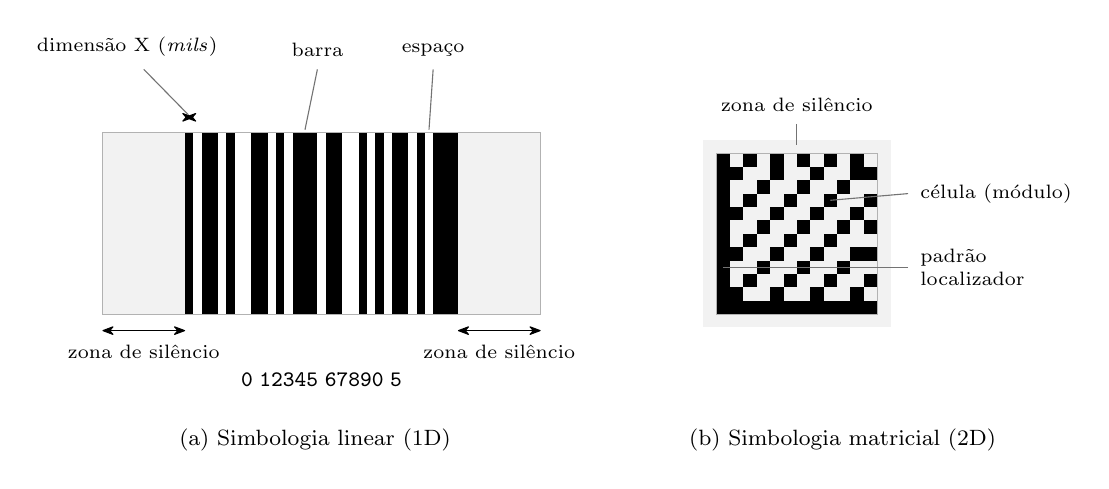
\begin{tikzpicture}[font=\footnotesize, >={Stealth[round]}]

% ---- (a) 1D linear ----
\begin{scope}[x=1.05mm,y=1.05mm]
	\fill[black!5] (0,0) rectangle (10,22);
	\fill[black!5] (43,0) rectangle (53,22);
	\foreach \bx/\bw in {10/1,12/2,15/1,18/2,21/1,23/3,27/2,31/1,33/1,35/2,38/1,40/3}
		\fill[black] (\bx,0) rectangle ({\bx+\bw},22);
	\draw[black!30] (0,0) rectangle (53,22);
	% anotações superiores
	\draw[<->] (10,23.8) -- (11,23.8);
	\node[font=\scriptsize, anchor=south] at (3,30) {dimensão X (\emph{mils})};
	\draw[black!55] (5,29.6) -- (10.4,24.1);
	\node[font=\scriptsize, anchor=south] at (26,30) {barra};
	\draw[black!55] (26,29.6) -- (24.5,22.3);
	\node[font=\scriptsize, anchor=south] at (40,30) {espaço};
	\draw[black!55] (40,29.6) -- (39.5,22.3);
	% anotações inferiores
	\draw[<->] (0,-2) -- (10,-2);
	\node[font=\scriptsize, anchor=north] at (5,-2.6) {zona de silêncio};
	\draw[<->] (43,-2) -- (53,-2);
	\node[font=\scriptsize, anchor=north] at (48,-2.6) {zona de silêncio};
	\node[font=\ttfamily\footnotesize] at (26.5,-8) {0\;12345\;67890\;5};
\end{scope}

% ---- (b) 2D matricial ----
\begin{scope}[xshift=78mm, x=1.7mm, y=1.7mm]
	\begin{scope}[on background layer]
		\fill[black!5] (-1,-1) rectangle (13,13);
	\end{scope}
	\foreach \i in {0,...,11}{
		\foreach \j in {0,...,11}{
			\pgfmathtruncatemacro{\cell}{ ( (\i==0) || (\j==0) || (\j==11 && mod(\i,2)==0) || (\i==11 && mod(\j,2)==0) || (\i>0 && \i<11 && \j>0 && \j<11 && mod(\i+2*\j,3)==0) ) ? 1 : 0 }
			\ifnum\cell=1 \fill[black] (\i,\j) rectangle ({\i+1},{\j+1}); \fi
		}
	}
	\draw[black!30] (0,0) rectangle (12,12);
	\node[font=\scriptsize, anchor=west] at (14.5,9) {célula (módulo)};
	\draw[black!55] (14.3,9) -- (8.5,8.5);
	\node[font=\scriptsize, anchor=west, align=left] at (14.5,3.5) {padrão\\localizador};
	\draw[black!55] (14.3,3.5) -- (0.5,3.5);
	\node[font=\scriptsize, anchor=south] at (6,14.4) {zona de silêncio};
	\draw[black!55] (6,14.2) -- (6,12.6);
\end{scope}

\node[font=\footnotesize] at (2.7,-1.6) {(a) Simbologia linear (1D)};
\node[font=\footnotesize] at (9.4,-1.6) {(b) Simbologia matricial (2D)};
\end{tikzpicture}

\vspace{4pt}
{\footnotesize Fonte: elaboração própria (2026).}
\end{figure}

A variedade de simbologias reflete diferentes compromissos entre tipo e volume de
dados, tamanho, densidade e setor de aplicação. O Quadro~\ref{qua-simbologias}
sintetiza as mais difundidas.

\begin{quadro}[htb]
\centering
\caption{Principais simbologias de código de barras}
\label{qua-simbologias}
\begin{tabular}{@{}p{2.5cm}p{1.6cm}p{2.1cm}p{3.5cm}p{2.0cm}@{}}
\toprule
\textbf{Simbologia} & \textbf{Categoria} & \textbf{Tipo de dado} & \textbf{Aplicação típica} & \textbf{Norma técnica}\\
\midrule
UPC-A / EAN-13 & Linear (1D) & Numérico & Varejo / ponto de venda (GS1) & GS1 Gen. Specs.\\
Code 39 & Linear (1D) & Alfanumérico & Industrial, defesa (MIL-STD-130) & ISO/IEC 16388\\
Code 128 & Linear (1D) & Alfanumérico (ASCII) & Logística e uso geral & ISO/IEC 15417\\
GS1-128 & Linear (1D) & Alfanumérico & Unidades logísticas / envio & ISO/IEC 15417 + GS1\\
ITF-14 & Linear (1D) & Numérico & Caixas e embalagens (DUN-14) & ISO/IEC 16390\\
GS1 DataBar & Linear (1D) & Numérico (GTIN) & Itens pequenos, perecíveis & GS1\\
PDF417 & 2D empilhada & Alfanum. / binário & Documentos, identidade, transporte & ISO/IEC 15438\\
Data Matrix & 2D matricial & Alfanum. / binário & Marcação de peças, saúde & ISO/IEC 16022\\
QR Code & 2D matricial & Alfanum. / binário & Consumo, \textit{mobile}, rastreio & ISO/IEC 18004\\
Aztec & 2D matricial & Alfanum. / binário & Bilhetagem, transporte & ISO/IEC 24778\\
\bottomrule
\end{tabular}

\vspace{2pt}
{\footnotesize Fonte: elaboração própria (2026), a partir de \citeonline{seagull}.}
\end{quadro}

Duas camadas de padronização coexistem. As \textbf{normas técnicas} especificam a
simbologia em si --- sua codificação e geometria (por exemplo, a ISO/IEC 15417 para
o Code~128 ou a ISO/IEC 16022 para o Data~Matrix) ---, enquanto as \textbf{normas de
aplicação}, independentes da simbologia, definem que dados e estrutura cada setor
exige \cite{seagull}. Sobre essa base atua o sistema \textbf{GS1}, cuja chave é o
\textbf{GTIN} (\textit{Global Trade Item Number}), descrito pela própria GS1 como
``a chave para gerenciar produtos em toda a cadeia de valor'', da fabricação ao
consumidor final \cite{gs1br}. Essa padronização resulta de décadas de trabalho de
organismos como UCC, ANSI, CEN, ISO/IEC e a AIM: a própria avaliação de qualidade
de impressão evoluiu do método ANSI (X3.182-1990) para a norma europeia EN~1635
(1995) e, então, para a internacional ISO/IEC 15416 (2000), todas partilhando a
mesma metodologia \cite{aim_layman} --- assunto aprofundado na
Seção~\ref{sec-qualidade}.

Esse arcabouço sustenta um alcance operacional vasto. A \textbf{precisão de dados} é
a motivação mais comum para adotar um sistema de código de barras: empresas com
leitura automatizada alcançam comumente \textbf{99\% de acurácia}, ante cerca de
85\% na entrada manual, aproximando-se da meta de 100\% exigida em contextos
críticos como hospitais e manufatura \cite{zebra_barcoding101}. A leitura óptica
funciona porque ``as barras pretas absorvem a luz e os espaços brancos a refletem''
\cite{gs1br}, convertendo em segundos uma ação física em transação digital. Ganhos
como acurácia, velocidade, rastreabilidade e controle de inventário explicam a
presença dos códigos de barras em praticamente todos os setores
(Quadro~\ref{qua-setores}).

\begin{quadro}[htb]
\centering
\caption{Setores e usos representativos da etiquetagem por código de barras}
\label{qua-setores}
\begin{tabular}{@{}p{3.6cm}p{8.4cm}@{}}
\toprule
\textbf{Setor} & \textbf{Uso representativo}\\
\midrule
Varejo & Ponto de venda, precisão de inventário e \textit{fulfillment} omnichannel\\
Transporte e logística & Comprovante de entrega, inventário de armazém e visibilidade da cadeia\\
Manufatura & Rastreio de produção (\textit{work-in-progress}) e rastreabilidade de peças\\
Saúde & Identificação de pacientes, amostras e medicamentos\\
Governo & Gestão de ativos, licenciamento e resposta a emergências\\
Energia e utilidades & Rastreio de ativos e ordens de serviço em campo\\
\bottomrule
\end{tabular}

\vspace{2pt}
{\footnotesize Fonte: elaboração própria (2026), a partir de \citeonline{zebra_industries} e \citeonline{gs1br}.}
\end{quadro}

Em todos esses cenários, contudo, o benefício depende de uma premissa simples: o
símbolo impresso precisa ser lido de forma confiável logo na primeira tentativa. A
leitura pressupõe que as proporções impressas correspondam às nominais; pequenos
desvios sistemáticos --- barras mais largas (\textbf{ganho}) ou mais estreitas
(\textbf{perda}) que o previsto --- comprometem a decodificação. É exatamente esse
tipo de desvio que a impressão térmica pode introduzir e cujo diagnóstico é o objeto
deste trabalho.

\subsection{Qualidade de impressão e verificação (ISO/IEC 15416 e 15415)}
\label{sec-qualidade}

A avaliação normativa parte do \textbf{perfil de refletância de varredura}
(\textit{scan reflectance profile}, SRP): uma linha de varredura atravessa o
símbolo medindo a refletância ao longo do percurso, produzindo uma curva de picos
(espaços claros) e vales (barras escuras). Todos os parâmetros de nota derivam
desse perfil \cite{iso15416}.

Para símbolos lineares, a ISO/IEC 15416 avalia nove atributos por varredura, entre
os quais se destacam os apresentados na Tabela~\ref{tab-iso}.

\begin{table}[htb]
\centering
\caption{Parâmetros de qualidade da ISO/IEC 15416 e sua relação com o defeito de
impressão}
\label{tab-iso}
\begin{tabular}{@{}p{3.4cm}p{4.6cm}p{5.2cm}@{}}
\toprule
\textbf{Parâmetro} & \textbf{O que mede} & \textbf{Relação com o defeito de impressão}\\
\midrule
Contraste do símbolo (SC) & Diferença entre a maior e a menor refletância &
Impressão clara ou mídia-\textit{ribbon} incompatível reduzem o contraste\\
Contraste de borda (EC) & Contraste entre barra e espaço adjacentes &
Bordas ``borradas'' por pressão/velocidade inadequadas\\
Modulação (MOD) & Uniformidade dos elementos ao longo do símbolo &
Pressão desigual e sujeira geram variação\\
Defeitos (ERN) & Maior não uniformidade de refletância de um elemento &
Manchas, \textit{voids} e pontos queimados\\
Decodificabilidade & Margem do símbolo frente ao algoritmo de referência &
Ganho/perda de largura das barras\\
\bottomrule
\end{tabular}

\vspace{2pt}
{\footnotesize Fonte: elaboração própria (2026), a partir de \citeonline{iso15416}.}
\end{table}

O ajuste de \textit{darkness} (temperatura da cabeça) é um dos fatores que mais
afetam esses parâmetros. A Figura~\ref{fig-darkness} ilustra a transição da
impressão clara demais (\textit{too light}), em que as barras finas desaparecem, à
escura demais (\textit{too dark}), em que barras e espaços se fundem, passando pela
faixa dentro da especificação (\textit{in spec}).

\begin{figure}[htb]
\centering
\caption{Efeito do \textit{darkness} na qualidade do código de barras: do claro demais (\textit{too light}) ao escuro demais (\textit{too dark})}
\label{fig-darkness}
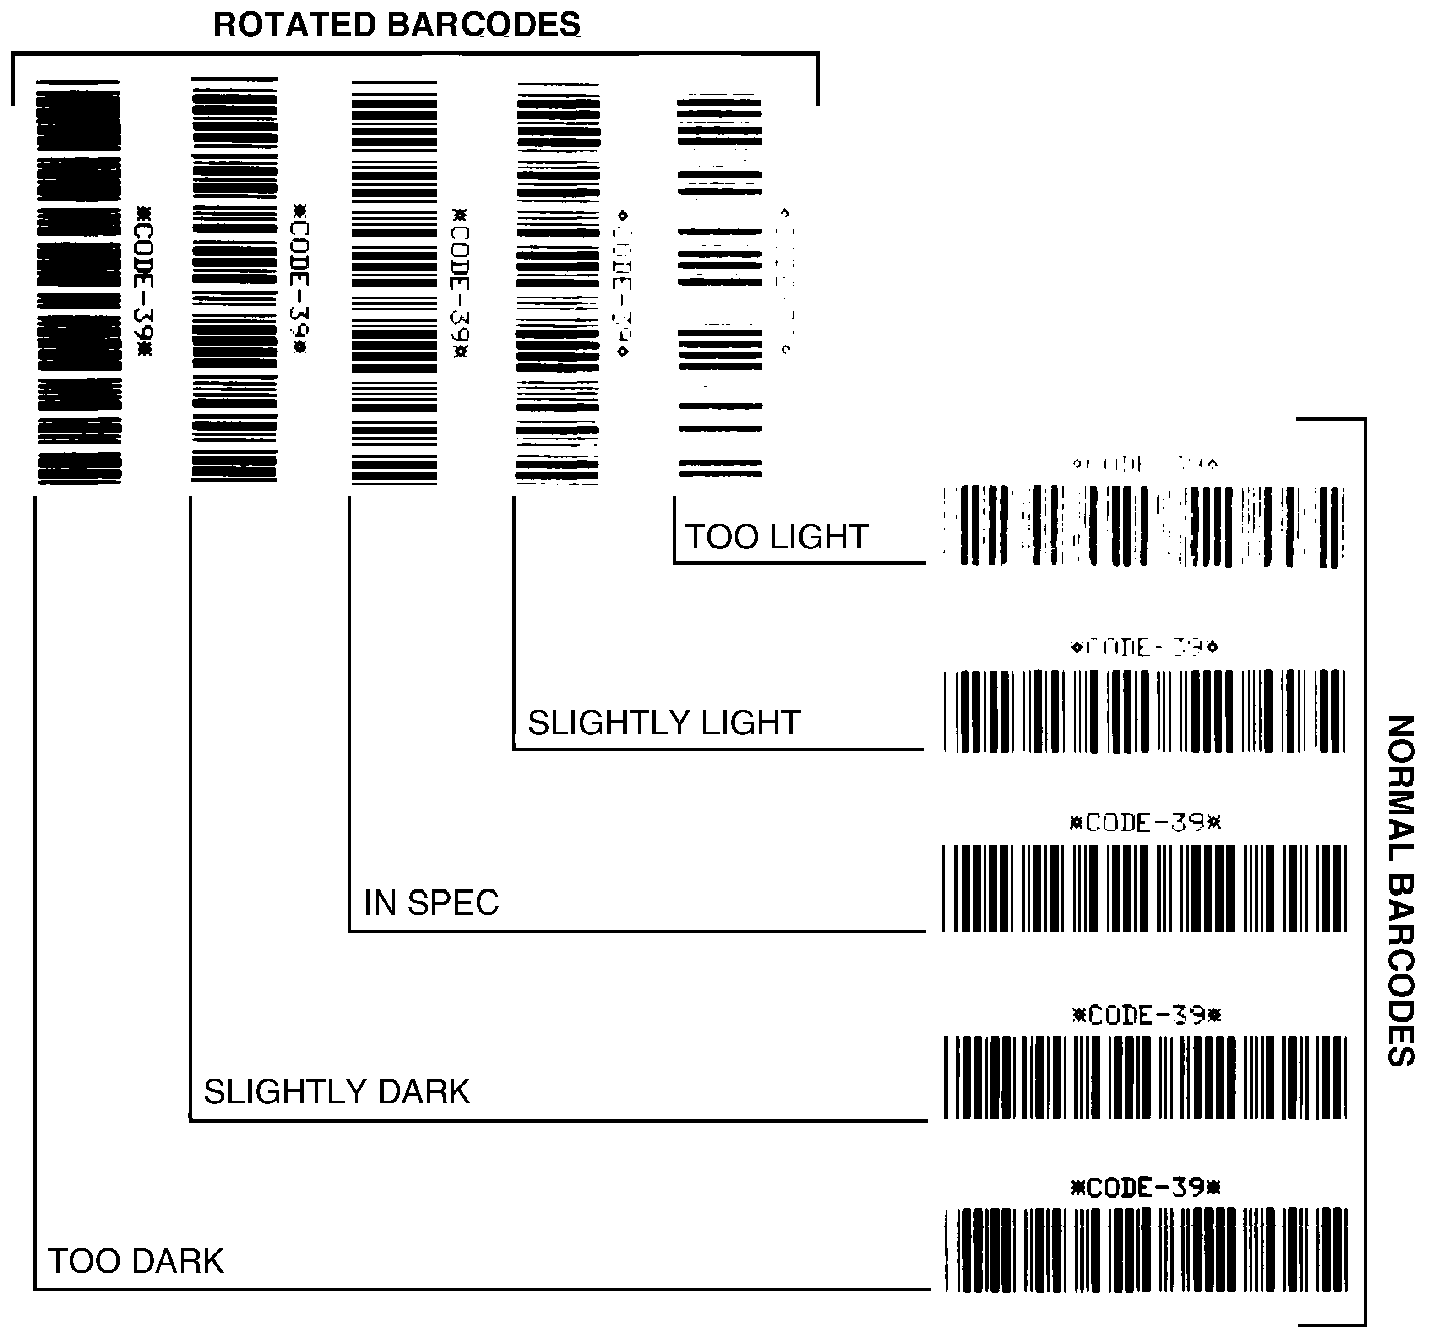
\includegraphics[width=0.82\textwidth]{figuras/zebra_darkness_comparison.png}

\vspace{2pt}
{\footnotesize Fonte: \citeonline{zebra_maintenance}.}
\end{figure}

A nota de uma varredura é a \textbf{menor} entre os parâmetros; a nota do símbolo
é a \textbf{média de dez varreduras} distribuídas ao longo da altura. Para 2D, a
ISO/IEC 15415 cumpre papel equivalente com parâmetros adaptados à matriz
\cite{iso15415}, e a marcação direta de peça (DPM) é tratada pela ISO/IEC 29158
\cite{iso29158}.

\noindent\textbf{Ponto metodológico importante.} A verificação \textit{conformante}
exige condições ópticas controladas --- fonte de luz definida, abertura de
medição, geometria e calibração de refletância --- providas por verificadores
certificados \cite{iso15426}. Uma imagem de câmera comum não reproduz essas
condições. Por isso, neste trabalho os parâmetros da norma são usados como
referencial conceitual e como indicadores aproximados, não como grau oficial ---
o que delimita honestamente o escopo (Seção~\ref{sec-fund}).

\subsection{Defeitos típicos de impressão térmica e suas causas}\label{sec-defeitos}

Impressoras térmicas de transferência (como a Zebra ZT411/ZT421) formam a imagem
aquecendo seletivamente uma cabeça de impressão que transfere tinta do
\textit{ribbon} para a mídia, prensada pelo rolete (\textit{platen}). Cada
componente falha de um modo com assinatura visual característica. A partir do guia
do usuário da ZT411/ZT421, do procedimento de manutenção e da base de
conhecimento da Zebra \cite{zebra_printquality}, consolida-se o mapeamento da
Tabela~\ref{tab-defeitos} --- que é, em si, uma das contribuições do trabalho.

\begin{table}[htb]
\centering
\caption{Mapeamento entre aparência do defeito, causa provável e ação corretiva}
\label{tab-defeitos}
\begin{tabular}{@{}p{4.4cm}p{4.2cm}p{4.6cm}@{}}
\toprule
\textbf{Defeito (aparência)} & \textbf{Causa provável} & \textbf{Ação corretiva típica}\\
\midrule
Código não escaneia; imagem ``suja'' & \textit{Darkness} alto demais ou pressão da
cabeça incorreta & Reduzir o \textit{darkness}; reduzir velocidade; ajustar pressão\\
Impressão clara (\textit{faded}) em toda a etiqueta & \textit{Darkness} baixo,
mídia/\textit{ribbon} incompatível ou alta velocidade & Elevar \textit{darkness};
trocar para combinação mídia-\textit{ribbon} adequada\\
Impressão clara/escura em um lado da etiqueta & Pressão \textbf{desigual} da cabeça
& Ajustar a pressão da cabeça (\textit{toggles})\\
Linhas cinza finas e angulares em etiquetas em branco & \textit{Ribbon} enrugado &
Corrigir tensão/alinhamento do \textit{ribbon}\\
Trilhas longas de impressão faltando & Elemento da cabeça danificado (linhas
brancas verticais) & Acionar assistência técnica (troca de cabeça)\\
\textit{Voids} no código; qualidade inconsistente & Cabeça de impressão \textbf{suja}
& Limpar cabeça e rolete com álcool isopropílico 99,7\%\\
Manchas (\textit{smudge}) & Mídia/\textit{ribbon} inadequados para alta velocidade
& Trocar por insumos recomendados\\
Perda de registro / deslocamento vertical & Rolete sujo, mídia mal carregada,
sensor descalibrado & Limpar rolete; recarregar mídia; calibrar sensores\\
\bottomrule
\end{tabular}

\vspace{2pt}
{\footnotesize Fonte: elaboração própria (2026), a partir de \citeonline{zebra_printquality}.}
\end{table}

A Figura~\ref{fig-defeitos-zebra} exemplifica, em etiquetas impressas reais, as
assinaturas visuais de vários desses defeitos, tal como documentadas pela Zebra
\cite{zebra_kb_printquality}. Note-se a correspondência com as classes reproduzidas
sinteticamente na Seção~\ref{sec-dados}.

\begin{figure}[htb]
\centering
\caption{Assinaturas visuais reais de defeitos de impressão térmica em etiquetas de códigos de barras}
\label{fig-defeitos-zebra}

\begin{minipage}[t]{0.31\textwidth}\centering
  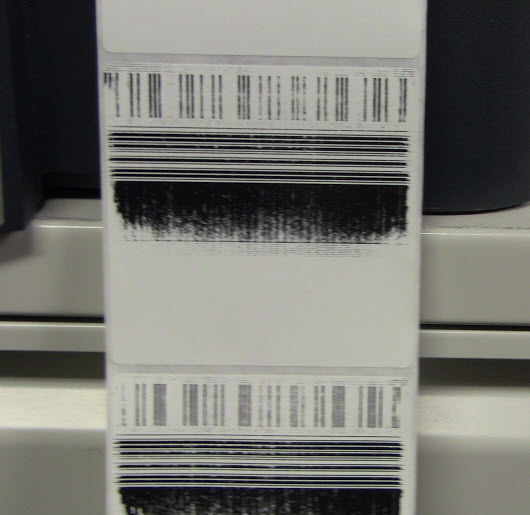
\includegraphics[width=\linewidth,height=3cm,keepaspectratio]{figuras/zebra_impressao_clara.jpg}\\[2pt]
  {\footnotesize (a) Impressão clara (\textit{faded})}
\end{minipage}\hfill
\begin{minipage}[t]{0.31\textwidth}\centering
  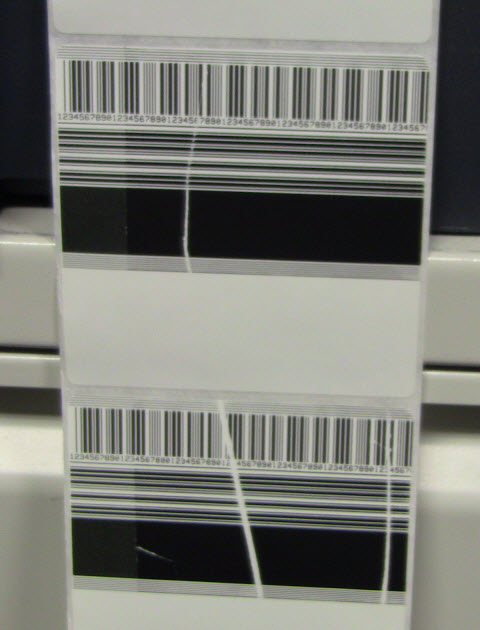
\includegraphics[width=\linewidth,height=3cm,keepaspectratio]{figuras/zebra_ribbon_enrugado.jpg}\\[2pt]
  {\footnotesize (b) \textit{Ribbon} enrugado}
\end{minipage}\hfill
\begin{minipage}[t]{0.31\textwidth}\centering
  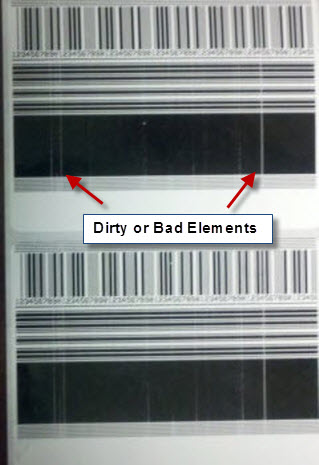
\includegraphics[width=\linewidth,height=3cm,keepaspectratio]{figuras/zebra_elemento_danificado.jpg}\\[2pt]
  {\footnotesize (c) Elemento da cabeça danificado}
\end{minipage}

\vspace{8pt}

\begin{minipage}[t]{0.31\textwidth}\centering
  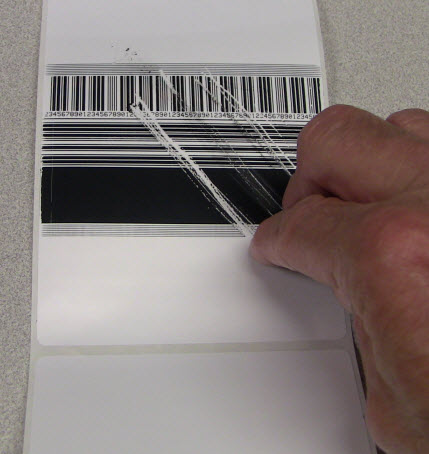
\includegraphics[width=\linewidth,height=3cm,keepaspectratio]{figuras/zebra_mancha.jpg}\\[2pt]
  {\footnotesize (d) Mancha (\textit{smear})}
\end{minipage}\hfill
\begin{minipage}[t]{0.31\textwidth}\centering
  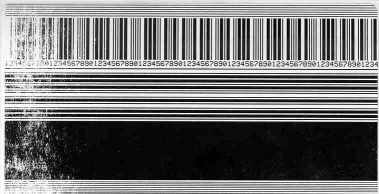
\includegraphics[width=\linewidth,height=3cm,keepaspectratio]{figuras/zebra_pressao_desigual.jpg}\\[2pt]
  {\footnotesize (e) Pressão desigual da cabeça}
\end{minipage}\hfill
\begin{minipage}[t]{0.31\textwidth}\centering
  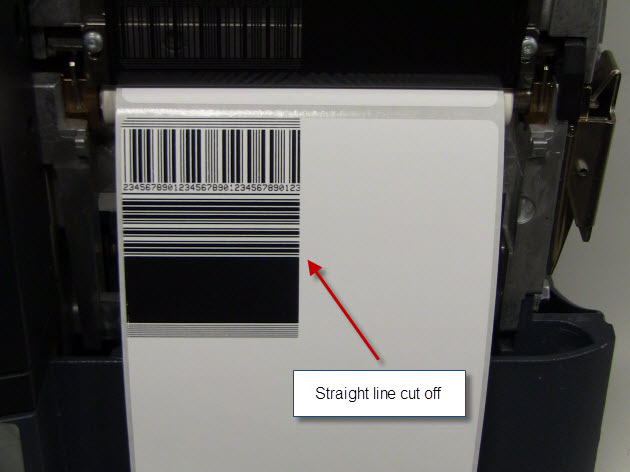
\includegraphics[width=\linewidth,height=3cm,keepaspectratio]{figuras/zebra_perda_registro.jpg}\\[2pt]
  {\footnotesize (f) Perda de registro (\textit{cutoff})}
\end{minipage}

\vspace{6pt}
{\footnotesize Fonte: \citeonline{zebra_kb_printquality}.}
\end{figure}

A manutenção preventiva atua sobre as causas de origem: a limpeza periódica da
cabeça e do rolete com álcool isopropílico 99,7\% (ou kit de manutenção Zebra) é
indicada quando surgem \textit{voids}, e a documentação alerta que
\textit{darkness} excessivo desgasta a cabeça prematuramente e pode ``queimar'' o
\textit{ribbon} \cite{zebra_printquality}. Esse conhecimento é o que alimenta o
agente de diagnóstico proposto na Seção~\ref{sec-proposta}.

\subsection{Processamento de imagens e visão computacional para inspeção}

O reconhecimento dos defeitos acima é um problema de \textbf{inspeção visual
automatizada}. As etapas clássicas envolvem:
\begin{alineas}
	\item \textbf{pré-processamento} --- conversão de cor, correção de iluminação
	e realce de contraste para atenuar variações de captura \cite{gonzalez2018};
	\item \textbf{localização/segmentação do símbolo} --- isolar a região do
	código na etiqueta, condição para medir refletância e detectar defeitos
	localizados \cite{szeliski2022};
	\item \textbf{detecção de objetos/defeitos} --- localizar e classificar
	regiões defeituosas; abordagens supervisionadas de um estágio (por exemplo, da
	família YOLO) são amplamente usadas em inspeção industrial;
	\item \textbf{classificação por redes convolucionais (CNN)} --- atribuir a
	classe de defeito a partir de características aprendidas, dispensando extração
	manual de atributos; e
	\item \textbf{detecção de anomalias} --- quando amostras de defeito real são
	escassas, métodos não supervisionados aprendem o ``normal'' e sinalizam
	desvios, contornando o desbalanceamento de dados.
\end{alineas}

A literatura recente de inspeção industrial converge nesses pilares e destaca um
desafio recorrente diretamente relevante a este trabalho: a \textbf{escassez de
imagens de defeito real}, que motiva aumento de dados e abordagens semi/não
supervisionadas \cite{frontiers2025anomaly,survey2022unsupervised}.

\subsection{Redes convolucionais, MobileNetV3 e transferência de aprendizado}
\label{sec-cnn}

Uma \textbf{rede neural convolucional} (CNN) aprende, camada a camada, filtros que
são convolvidos com a imagem para produzir \textit{mapas de características}
(\textit{feature maps}). As primeiras camadas respondem a padrões genéricos ---
bordas, cantos e texturas ---, enquanto as camadas profundas combinam esses padrões
em conceitos específicos da tarefa; é essa hierarquia que dispensa a extração manual
de atributos \cite{gonzalez2018,szeliski2022}. Como as camadas iniciais aprendem
características transferíveis entre domínios, é possível reaproveitar uma rede
pré-treinada em um grande conjunto (ImageNet) e apenas \textbf{ajustá-la}
(\textit{fine-tuning}) à tarefa-alvo --- estratégia de \textbf{transferência de
aprendizado} que melhora a generalização quando há poucos dados rotulados
\cite{yosinski2014transferable}.

Adota-se a \textbf{MobileNetV3-Small} \cite{howard2019mobilenetv3}, projetada para
ser leve e eficiente. Três elementos explicam sua economia: (i) \textbf{convoluções
separáveis em profundidade} (\textit{depthwise separable}), que fatoram a convolução
padrão em um filtro espacial por canal seguido de uma combinação $1\times1$,
reduzindo drasticamente parâmetros e operações; (ii) blocos \textbf{Squeeze-and-Excitation},
um mecanismo de atenção que reponderar canais conforme sua relevância; e (iii) a
não linearidade \textbf{h-swish}, aproximação barata do \textit{swish}. O resultado é
uma rede de $\approx$1,5~milhão de parâmetros que treina e infere bem mesmo em CPU
--- adequada ao objetivo de baixo custo deste trabalho. Como \textit{baselines} de
comparação (Seção~\ref{sec-resultados}) empregam-se a \textbf{ResNet18}
\cite{he2016resnet}, que populariza as conexões residuais, e a \textbf{EfficientNet-B0}
\cite{tan2019efficientnet}, que escala profundidade, largura e resolução de forma
balanceada.

\noindent\textbf{Generalização com poucos dados.} Treinar em um conjunto pequeno
favorece o \textit{overfitting} (o modelo memoriza o treino e não generaliza). Três
mecanismos o mitigam aqui: a transferência de aprendizado (reduz os parâmetros
efetivamente estimados do zero), o \textbf{aumento de dados} (\textit{data
augmentation}) --- rotações e variações de brilho/contraste que ampliam a
variabilidade sem alterar o rótulo \cite{shorten2019augmentation} --- e a própria
arquitetura leve, de menor capacidade. A avaliação por \textbf{validação cruzada}
(Seção~\ref{sec-resultados}) complementa essas medidas ao estimar o desempenho de
forma menos sensível a uma única partição.

\subsection{Sistemas multiagentes e o \textit{Agent Development Kit} (ADK)}

Um \textbf{sistema multiagente} é um conjunto de agentes autônomos que colaboram
para uma meta comum, cada um responsável por uma subtarefa. O \textit{Agent
Development Kit} (ADK), apresentado pelo Google no Cloud NEXT 2025, é um
\textit{framework} de código aberto para construir e orquestrar esses sistemas
\cite{google_adk_blog}. Ele organiza os agentes em três tipos:
\begin{alineas}
	\item \textbf{agentes LLM} --- o ``raciocínio'', que interpreta entradas e
	decide ações;
	\item \textbf{agentes de \textit{workflow}} --- orquestradores de fluxo
	(sequencial, paralelo, em laço); e
	\item \textbf{agentes customizados} --- especialistas que encapsulam lógica ou
	modelos próprios (por exemplo, um modelo de visão).
\end{alineas}

Os agentes se organizam em uma \textbf{hierarquia} e se comunicam por estado
compartilhado, delegação e invocação explícita \cite{adk_docs}. A justificativa
central do paradigma --- que motiva a arquitetura adotada neste trabalho --- é que
decompor um problema em agentes especializados tende a ser mais confiável, modular
e manutenível do que um único modelo/prompt monolítico, porque cada agente resolve
uma tarefa mais simples e bem delimitada.

% ---------------------------------------------------------------------------
\section{Trabalhos relacionados}\label{sec-relacionados}
% ---------------------------------------------------------------------------

\subsection{Verificação normativa e diagnóstico de defeitos}

A base da verificação de qualidade são as normas ISO/IEC 15416 e 15415,
implementadas por verificadores comerciais que reportam notas A--F
\cite{iso15416,iso15415}. Há também soluções que inferem falhas do mecanismo de
impressão a partir da própria leitura --- por exemplo, detectando linhas não
impressas para gerar um relatório de manutenção do cabeçote e alertar antes da
falha total \cite{patent9826106}. \textbf{Limitação comum:} dependem de
\textit{hardware} dedicado e/ou entregam a nota/alerta, sem um diagnóstico de
causa-raiz acionável e contextualizado pela documentação do fabricante.

\subsection{Inspeção visual de defeitos com aprendizado profundo}

A inspeção industrial baseada em aprendizado profundo é sistematizada em
levantamentos recentes que cobrem CNNs, detecção de objetos e detecção de
anomalias, com ênfase no problema de dados escassos
\cite{frontiers2025anomaly,survey2022unsupervised}. Aplicações diretas ao domínio
de impressão incluem a detecção de defeitos em tecidos estampados com CNN
\cite{fabric2021cnn} e a detecção/localização de anomalias em manufatura aditiva
por transferência de aprendizado \cite{fff2024thermal}. \textbf{Limitação comum:}
focam a classificação/localização do defeito visual, sem ligá-lo à causa física
do processo nem a uma ação corretiva.

\subsection{Sistemas multiagentes aplicados a tarefas de visão}

A orquestração multiagente com ADK e \textit{frameworks} correlatos vem sendo
aplicada a tarefas complexas que se beneficiam de decomposição, tratando agentes
especializados como ferramentas de um agente raiz \cite{google_adk_blog}.
\textbf{Lacuna observada:} a combinação de orquestração multiagente com inspeção
de qualidade de impressão de códigos de barras --- em especial acoplando detecção
visual a diagnóstico fundamentado em documentação técnica --- é pouco explorada.

\subsection{Lacuna que este trabalho preenche}

Reunindo os três eixos: os verificadores dão nota mas não causa; os métodos de
visão detectam o defeito mas não a causa nem a correção; e a orquestração
multiagente é madura porém raramente aplicada a este domínio. Este trabalho se
posiciona nessa interseção, propondo um sistema de baixo custo, servido por API,
que combina estimativa de indicadores de qualidade, detecção visual de defeitos
físicos e diagnóstico de causa-raiz fundamentado na documentação da Zebra,
orquestrados por agentes especializados. O Quadro comparativo da
Tabela~\ref{tab-comparativo} posiciona este trabalho frente às abordagens
existentes.

\begin{table}[htb]
\centering
\caption{Comparativo entre abordagens quanto aos recursos oferecidos}
\label{tab-comparativo}
\begin{tabular}{@{}p{4.2cm}*{4}{>{\centering\arraybackslash}p{2.2cm}}@{}}
\toprule
\textbf{Abordagem} & \textbf{Nota ISO} & \textbf{Defeito físico} &
\textbf{Causa-raiz} & \textbf{Sem \textit{hardware} dedicado}\\
\midrule
Verificadores certificados & Sim & Não & Não & Não\\
Visão computacional (CNN/anomalia) & Não & Sim & Não & Sim\\
Detecção via leitura (patente) & Parcial & Parcial & Parcial & Não\\
\textbf{Este trabalho} & Aprox. & Sim & Sim & Sim\\
\bottomrule
\end{tabular}

\vspace{2pt}
{\footnotesize Fonte: elaboração própria (2026).}
\end{table}

\subsection{Comparação explícita com \textit{Research on a Multi-Type Barcode Defect Detection Model Based on Machine Vision}}\label{sec-sota}

Recentemente, Duan et al.~\cite{duan2025barcode} propuseram um sistema de
detecção de defeitos em códigos de barras baseado em uma arquitetura em dois
estágios composta por YOLOv8n e uma rede híbrida ResNet50--ViT (denominada
\textbf{Y8-LiBARNet}), treinada sobre o conjunto público \textbf{BarBeR}. Embora o
método apresente elevada precisão na localização e classificação de códigos
defeituosos, sua saída limita-se à identificação do estado do código (íntegro ou
defeituoso), sem estabelecer relação entre o defeito observado, sua provável causa
física e a ação corretiva correspondente. O presente trabalho complementa essa
lacuna ao integrar classificação visual, diagnóstico fundamentado na documentação
técnica do fabricante e orquestração multiagente para apoio à manutenção
industrial. Os dois trabalhos atacam problemas parecidos, mas por
\textbf{perspectivas diferentes}, o que reduz a sobreposição científica; a
Tabela~\ref{tab-sota-qual} confronta ambos por aspecto.

\begin{table}[htb]
\centering
\caption{Comparação por aspecto entre este trabalho e Duan et al. (2025)}
\label{tab-sota-qual}
\footnotesize
\begin{tabular}{@{}p{2.5cm}p{5.4cm}p{5.4cm}@{}}
\toprule
\textbf{Aspecto} & \textbf{Este trabalho} & \textbf{Duan et al. \cite{duan2025barcode}}\\
\midrule
Objetivo & Diagnosticar defeitos de impressão e sugerir a causa física &
Detectar códigos e classificar se possuem defeito\\
Entrada & Foto de uma etiqueta & Foto contendo um ou mais códigos\\
\textit{Pipeline} & OpenCV $+$ CNN $+$ multiagentes $+$ RAG &
YOLOv8 $+$ ResNet50 $+$ ViT\\
Saída & Defeito $+$ causa $+$ ação corretiva &
Localização $+$ classe (íntegro/defeituoso)\\
Foco & Apoio à manutenção da impressora & Inspeção industrial automática\\
\textit{Hardware} alvo & CPU comum (sem GPU) & GPU dedicada (RTX 4060 nos experimentos)\\
\textit{Dataset} & Defeitos sintéticos sobre códigos-base públicos (BarBeR/Roboflow) $+$ imagens reais próprias &
BarBeR (8.748 imagens públicas, com rótulos reais)\\
\bottomrule
\end{tabular}

\vspace{2pt}
{\footnotesize Fonte: elaboração própria (2026).}
\end{table}

\noindent\textbf{Onde o método de Duan et al.\ é mais forte.} Há pontos em que
aquele trabalho é objetivamente superior. \textbf{(i) \textit{Dataset}:}
utilizam cerca de 8.748 imagens do BarBeR, contemplando 18 simbologias, códigos
1D e 2D, iluminação variada, superfícies planas e curvas e diferentes sensores,
\textbf{com rótulos reais de defeito}; este trabalho apoia-se em 52 imagens reais
somadas ao conjunto sintético de defeitos --- este último gerado sobre
códigos-base limpos das mesmas bases públicas (BarBeR \cite{2024ICPR_barber} e
Roboflow \cite{roboflow_barcode}), porém \textbf{sem herdar seus rótulos} ---,
totalizando cerca de 630 imagens para treino/teste da CNN --- provável
primeiro ponto a ser observado por um revisor. \textbf{(ii) Arquitetura:} adotam
um \textit{pipeline} de dois estágios mais sofisticado
(Figura~\ref{fig-pipelines}), ao passo que a proposta aqui é deliberadamente mais
simples, priorizando baixo custo. \textbf{(iii) Resultados:} reportam valores
superiores em termos absolutos (Tabela~\ref{tab-sota-quant}). À primeira vista o
desempenho parece inferior, mas a comparação direta seria injusta, pois as
\textbf{tarefas são distintas} --- decidir a \emph{presença} do defeito em
imagens reais \textit{versus} classificar a \emph{causa} física sobre um conjunto
sintético.

\noindent\textbf{Onde este trabalho é mais forte.} A maior oportunidade está no
escopo. \textbf{(i) Problema distinto:} enquanto o trabalho de referência
responde ``\emph{existe} defeito?'', este responde ``\emph{qual} defeito é este?''
e, além disso, ``\emph{qual componente} da impressora provavelmente o causou?''
--- passo que simplesmente não existe no trabalho comparado.
\textbf{(ii) Diagnóstico de causa-raiz:} este é o principal diferencial. A
solução mapeia imagem $\rightarrow$ classe do defeito $\rightarrow$ documentação
Zebra $\rightarrow$ causa provável $\rightarrow$ ação corretiva
(Figura~\ref{fig-causaraiz}), aproximando-se de um sistema especialista apoiado
por IA; o trabalho de Duan et al.\ encerra-se na classificação.
\textbf{(iii) Orquestração multiagente:} não há, naquele trabalho, equivalente ao
\textit{pipeline} de agentes especializados (leitura $\rightarrow$ indicadores
$\rightarrow$ CNN $\rightarrow$ RAG $\rightarrow$ laudo) da
Figura~\ref{fig-arquitetura}, que converte um classificador em um sistema de
apoio à decisão. \textbf{(iv) Interpretabilidade e custo:} o sistema explica por que
detectou o defeito, qual documento sustentou a conclusão, qual componente trocar
e qual ajuste fazer --- informação de valor industrial direto --- e o faz em
\textbf{CPU comum, sem GPU}, ao passo que o trabalho de referência recorre a uma
GPU dedicada (RTX 4060); a viabilidade em hardware modesto é, por si só, um
diferencial para o cenário de baixo custo visado aqui.

\begin{figure}[htb]
\centering
\caption{Contraste entre os \textit{pipelines}: Duan et al.\ (dois estágios) e este trabalho}
\label{fig-pipelines}
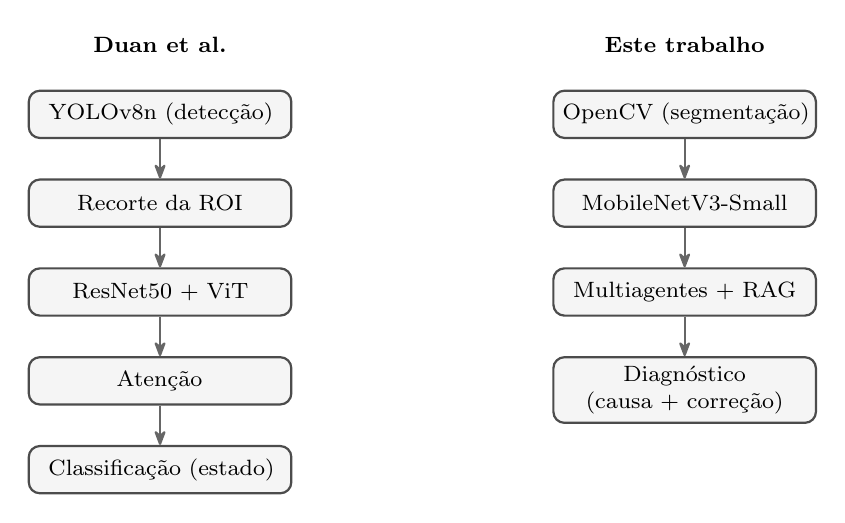
\begin{tikzpicture}[
	font=\footnotesize,
	>={Stealth[round]},
	node distance=0.5cm,
	et/.style={rectangle, rounded corners, draw=black!70, fill=black!4, thick, text width=3.1cm, minimum height=0.6cm, align=center},
	tit/.style={font=\footnotesize\bfseries},
	seta/.style={->, thick, black!60},
]
% Coluna esquerda: Duan et al.
\node[et] (a1) {YOLOv8n (detecção)};
\node[et] (a2) [below=of a1] {Recorte da ROI};
\node[et] (a3) [below=of a2] {ResNet50 $+$ ViT};
\node[et] (a4) [below=of a3] {Atenção};
\node[et] (a5) [below=of a4] {Classificação (estado)};
\node[tit] [above=0.35cm of a1] {Duan et al.};
\draw[seta] (a1)--(a2); \draw[seta] (a2)--(a3); \draw[seta] (a3)--(a4); \draw[seta] (a4)--(a5);
% Coluna direita: este trabalho
\node[et] (b1) [right=3.3cm of a1] {OpenCV (segmentação)};
\node[et] (b2) [below=of b1] {MobileNetV3-Small};
\node[et] (b3) [below=of b2] {Multiagentes $+$ RAG};
\node[et] (b4) [below=of b3] {Diagnóstico (causa $+$ correção)};
\node[tit] [above=0.35cm of b1] {Este trabalho};
\draw[seta] (b1)--(b2); \draw[seta] (b2)--(b3); \draw[seta] (b3)--(b4);
\end{tikzpicture}

\vspace{2pt}
{\footnotesize Fonte: elaboração própria (2026).}
\end{figure}

\begin{table}[htb]
\centering
\caption{Comparação quantitativa (valores absolutos; tarefas e dados \emph{distintos})}
\label{tab-sota-quant}
\footnotesize
\begin{tabular}{@{}p{3.0cm}p{3.6cm}p{2.4cm}p{2.3cm}c@{}}
\toprule
\textbf{Trabalho} & \textbf{Tarefa} & \textbf{Dataset} & \textbf{Métrica} & \textbf{Valor}\\
\midrule
Duan et al. \cite{duan2025barcode} & Localização & BarBeR (real) & mAP@0,5 & 0,984\\
Duan et al. \cite{duan2025barcode} & Classificação & BarBeR (real) & Acurácia / F1 & 0,925 / 0,919\\
\textbf{Este trabalho} & Classificação (7 causas) & Sintético & Acurácia / Macro-F1 & 0,84 / 0,84\\
\bottomrule
\end{tabular}

\vspace{2pt}
{\footnotesize Fonte: elaboração própria (2026). A comparação direta seria
injusta: as tarefas (\emph{presença} \textit{vs.} \emph{causa} do defeito), os
conjuntos (real \textit{vs.} sintético) e o \textit{hardware} (GPU \textit{vs.}
CPU) diferem; os valores apenas situam a ordem de grandeza.}
\end{table}

\begin{figure}[htb]
\centering
\caption{Cadeia de diagnóstico de causa-raiz que estende a classificação --- ausente em Duan et al.}
\label{fig-causaraiz}
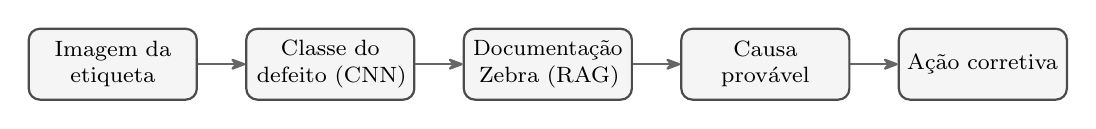
\begin{tikzpicture}[
	font=\footnotesize,
	>={Stealth[round]},
	no/.style={rectangle, rounded corners, draw=black!70, fill=black!4, thick, text width=1.9cm, minimum height=0.9cm, align=center},
	seta/.style={->, thick, black!60},
]
\node[no] (i) {Imagem da etiqueta};
\node[no] (c) [right=0.6cm of i] {Classe do defeito (CNN)};
\node[no] (m) [right=0.6cm of c] {Documentação Zebra (RAG)};
\node[no] (ca) [right=0.6cm of m] {Causa provável};
\node[no] (ac) [right=0.6cm of ca] {Ação corretiva};
\draw[seta] (i)--(c); \draw[seta] (c)--(m); \draw[seta] (m)--(ca); \draw[seta] (ca)--(ac);
\end{tikzpicture}

\vspace{2pt}
{\footnotesize Fonte: elaboração própria (2026).}
\end{figure}

\noindent\textbf{Comparando apenas o classificador.} A escolha do \textit{backbone}
apoiou-se em uma etapa de \textbf{seleção de modelos} executada durante a
construção deste trabalho (revisão~V2, 15 jul.\ 2026), sobre o conjunto sintético
(Seção~\ref{sec-dados}). Três arquiteturas foram treinadas e avaliadas sob
\emph{protocolo idêntico} --- mesmos dados, augmentação e hiperparâmetros ---, com
\textit{tuning} e treinamento completos; a Tabela~\ref{tab-sota-cnn} resume os
resultados atingidos. Esse é um rigor experimental frequentemente ausente em
trabalhos aplicados, e a análise completa consta da Seção~\ref{sec-comparacao}.

\begin{table}[htb]
\centering
\caption{Comparação de arquiteturas do classificador no teste fixo (protocolo idêntico)}
\label{tab-sota-cnn}
\begin{tabular}{@{}lcccc@{}}
\toprule
\textbf{Modelo} & \textbf{Acurácia} & \textbf{Macro-F1} & \textbf{Parâmetros (M)} & \textbf{Latência (ms)}\\
\midrule
\textbf{MobileNetV3-Small (adotado)} & \textbf{0,84} & \textbf{0,84} & 1,5 & 4,5\\
ResNet18 & 0,79 & 0,80 & 11,2 & 17,8\\
EfficientNet-B0 & 0,90 & 0,89 & 4,0 & 16,5\\
\bottomrule
\end{tabular}

\vspace{2pt}
{\footnotesize Fonte: elaboração própria (2026). Etapa de seleção de modelos
(revisão~V2, 15 jul.\ 2026). Latência média por imagem em CPU.}
\end{table}

\begin{alineas}
	\item \textbf{significância estatística (McNemar):} nenhuma diferença é
	significativa ao nível de 5\% --- MobileNetV3-Small \textit{vs.}
	EfficientNet-B0 ($b{=}4$, $c{=}10$, $p{=}0{,}18$) e \textit{vs.} ResNet18
	($b{=}10$, $c{=}5$, $p{=}0{,}30$). Ou seja, no conjunto de teste disponível não
	há evidência de que a EfficientNet-B0 seja superior; somado à sua eficiência
	muito maior, isso sustenta a escolha da MobileNetV3-Small para o cenário de
	baixo custo;
	\item \textbf{validação cruzada (5 dobras estratificadas):} a MobileNetV3-Small
	obteve acurácia de 0,82\,$\pm$\,0,01 e Macro-F1 de 0,82\,$\pm$\,0,02,
	indicando desempenho estável e pouco sensível à partição; e
	\item \textbf{ponto fraco:} confusão mútua entre \emph{sem defeito} e
	\emph{cabeça queimada} (F1~$\approx$~0,56) --- as zonas claras entre as barras
	imitam as linhas brancas verticais do dano na cabeça.
\end{alineas}

\noindent Novos testes, após \textit{tuning} e treinamento, confirmaram esses
resultados, consolidando a MobileNetV3-Small como o modelo adotado no trabalho.

\noindent\textbf{Síntese.} Em síntese, os dois trabalhos são
\textbf{complementares}: o de Duan et al.\ é mais forte em detecção visual e
validação em larga escala, enquanto este se destaca por transformar a
classificação em um sistema de apoio à manutenção, combinando visão computacional,
conhecimento técnico do fabricante e orquestração multiagente. Esse posicionamento
constitui um diferencial claro, retomado na discussão dos resultados
(Seção~\ref{sec-resultados}). Uma comparação \emph{indireta} e mais justa passa por
avaliar o classificador sobre o próprio BarBeR (experimento~E4,
Seção~\ref{sec-baseline}).

% ---------------------------------------------------------------------------
\section{Metodologia}\label{sec-metodo}
% ---------------------------------------------------------------------------

\subsection{Tipo de pesquisa}

Pesquisa de natureza \textbf{aplicada}, abordagem \textbf{quantitativa} e objetivo
\textbf{exploratório-experimental}: constrói-se um artefato (o sistema) e mede-se
seu desempenho em condições controladas, com procedimento experimental.

\subsection{Conjunto de dados}\label{sec-dados}

O problema tem duas naturezas distintas --- a \textbf{legibilidade da captura} (a
imagem do código está boa o suficiente para ler?) e o \textbf{defeito de
impressão} (que falha do processo produziu a marca?) --- e cada uma exige um tipo
de dado. Por isso, adota-se uma estratégia de \textbf{duas trilhas}.

\noindent\textbf{Trilha A --- imagens reais de captura (base disponível).}
Conjunto de 52 imagens reais de códigos de barras fotografados em produtos e
embalagens, em tons de cinza, sob ângulo, reflexo, curvatura e fundos variados, já
organizadas por simbologia, conforme a Tabela~\ref{tab-trilhaA}. Esse conjunto é
usado para treinar/avaliar o agente de leitura/decodificação e o agente de
indicadores de legibilidade. Como são todas 1D, as amostras 2D são complementadas
na Trilha B.

\begin{table}[htb]
\centering
\caption{Trilha A --- imagens reais por simbologia}
\label{tab-trilhaA}
\begin{tabular}{@{}lc@{}}
\toprule
\textbf{Simbologia} & \textbf{N.º de imagens}\\
\midrule
EAN-13 & 19\\
Code 39 & 6\\
Code 128 & 5\\
EAN-8 & 5\\
\textit{Interleaved 2 of 5} & 5\\
EAN-13 (\textit{add-on} 2) & 4\\
EAN-13 (\textit{add-on} 5) & 4\\
Pharmacode & 4\\
\midrule
\textbf{Total} & \textbf{52}\\
\bottomrule
\end{tabular}

\vspace{2pt}
{\footnotesize Fonte: elaboração própria (2026).}
\end{table}

\noindent\textbf{Trilha B --- defeitos de impressão sintéticos (gerados).} Para
treinar o agente de defeitos físicos não há um conjunto público rotulado de
defeitos de impressão térmica, e as fotos da base de conhecimento da Zebra são
material protegido por direitos autorais. Adota-se, então, \textbf{geração
sintética controlada}: a partir de \textbf{códigos de barras limpos (1D e 2D)}
--- extraídos de bases públicas de imagens reais, o repositório de
\textit{benchmarking} \textbf{BarBeR} \cite{2024ICPR_barber,2025EAAI} e projetos
do \textbf{Roboflow Universe} \cite{roboflow_barcode} --- aplicam-se
transformações que reproduzem a assinatura visual de cada defeito descrito na
documentação Zebra \cite{zebra_printquality}, conforme a Tabela~\ref{tab-trilhaB}.
As imagens dessas bases entram \textbf{exclusivamente como códigos-base limpos}
(substrato) sobre os quais o gerador injeta os defeitos; \textbf{nenhum rótulo de
defeito é herdado} dessas fontes.
Um gerador de referência foi implementado (\texttt{generate\_dataset.py}) e produz as
sete classes de forma balanceada, com divisão automática em treino/validação/teste
(70/15/15) e parâmetros de defeito amostrados aleatoriamente em faixas definidas.
A Figura~\ref{fig-dataset} ilustra amostras das classes geradas.

\begin{table}[htb]
\centering
\caption{Trilha B --- classes de defeito e transformação sintética correspondente}
\label{tab-trilhaB}
\begin{tabular}{@{}p{4.6cm}p{5.0cm}p{4.0cm}@{}}
\toprule
\textbf{Classe de defeito} & \textbf{Transformação sintética} & \textbf{Sintoma reproduzido}\\
\midrule
Cabeça queimada (elemento danificado) & Linhas brancas verticais contínuas &
Trilhas longas de impressão faltando\\
\textit{Ribbon} enrugado & Faixas claras finas e diagonais & Linhas cinza angulares\\
Ponto queimado / \textit{darkness} alto & Manchas escuras localizadas &
Excesso de temperatura\\
Impressão clara (\textit{darkness} baixo) & Redução de contraste global &
\textit{Faded} / mídia-\textit{ribbon} incompatível\\
Pressão desigual & Borrão direcional (gradiente em um lado) & Densidade não uniforme\\
Cabeça suja (\textit{voids}) & Falhas brancas pontuais nas barras & \textit{Voids} no código\\
Sem defeito & (código limpo) & Classe de controle\\
\bottomrule
\end{tabular}

\vspace{2pt}
{\footnotesize Fonte: elaboração própria (2026).}
\end{table}

\begin{figure}[htb]
\centering
\caption{Amostras do conjunto sintético de defeitos, uma classe por bloco}
\label{fig-dataset}
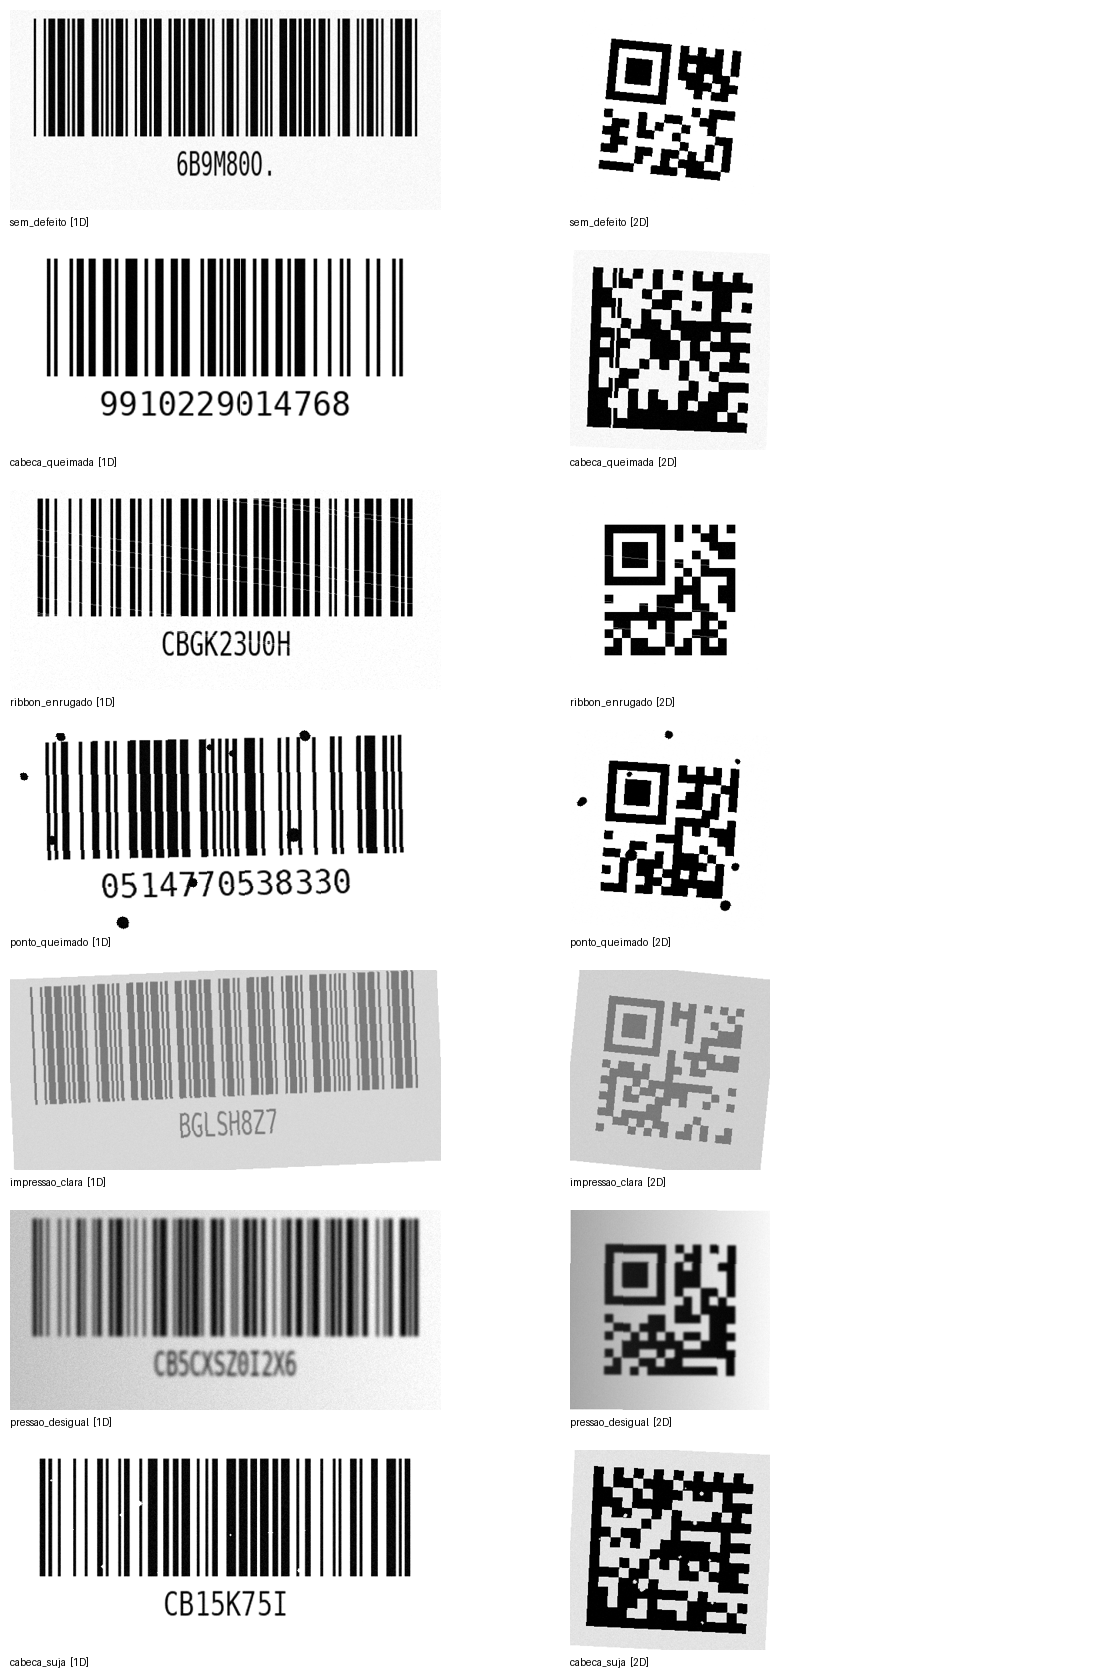
\includegraphics[width=0.95\textwidth]{figuras/dataset_preview.png}

\vspace{2pt}
{\footnotesize Fonte: elaboração própria (2026), gerada por \texttt{generate\_dataset.py}.}
\end{figure}

Essa abordagem é reprodutível, balanceável e livre de restrições autorais, e é
prática consolidada na literatura de inspeção quando amostras reais são escassas
\cite{frontiers2025anomaly,survey2022unsupervised}.

\noindent\textbf{Divisão e aumento de dados.} Cada trilha é dividida em
treino/validação/teste (70/15/15), estratificando por classe. Sobre a Trilha A
aplica-se aumento de dados clássico (rotação, variação de brilho/contraste,
recortes) para ampliar a variabilidade de captura. Os parâmetros dos defeitos
sintéticos (intensidade, quantidade, posição) são amostrados aleatoriamente em
faixas definidas, para evitar que o modelo aprenda um padrão fixo.

\noindent\textbf{Datasets externos e proveniência das imagens-base.} Os
códigos-base limpos da Trilha~B provêm de duas fontes públicas de imagens reais
de códigos de barras: o repositório de \textit{benchmarking} \textbf{BarBeR}
\cite{2024ICPR_barber,2025EAAI} e projetos do \textbf{Roboflow Universe}
\cite{roboflow_barcode}. Em ambos os casos as imagens entram \textbf{apenas como
substrato limpo} para a síntese de defeitos (papel \texttt{bases}); opcionalmente,
uma partição real é reservada como \textbf{conjunto de teste de generalização}
(sintético $\rightarrow$ real, papel \texttt{test}), nunca misturada ao treino. O
projeto inclui um utilitário de \textit{download} reprodutível --- por exemplo,
para baixar e recortar os códigos-base de um projeto do Roboflow:

\begin{quote}\footnotesize\ttfamily
python -m config.download\_roboflow --workspace o-xfs34\\
\hspace*{2em}--project barcode-detection-tvdug --version 1\\
\hspace*{2em}--role bases --symbology mixed --crop
\end{quote}

\noindent\textbf{Licenciamento das imagens.} As imagens são utilizadas \textbf{em
conformidade com as licenças declaradas nas respectivas fontes}: a licença do
repositório BarBeR \cite{2024ICPR_barber,2025EAAI} e a licença de cada projeto do
Roboflow Universe --- majoritariamente \textit{Creative Commons} CC~BY~4.0,
verificada projeto a projeto na página de origem \cite{roboflow_barcode}. O uso
restringe-se a \textbf{códigos-base para geração sintética de defeitos}, com a
devida atribuição aos autores e sem redistribuição das imagens originais.

\subsection{Ferramentas utilizadas}

\begin{alineas}
	\item \textbf{visão computacional:} Python, OpenCV e \textbf{PyTorch}. O
	PyTorch é hoje o \textit{framework} predominante na comunidade acadêmica, o
	que favorece a reprodutibilidade e a comparação com trabalhos correlatos. Para
	atender a máquinas modestas, adota-se transferência de aprendizado com o
	\textit{backbone} leve \textbf{MobileNetV3-Small} (ResNet18 e EfficientNet-B0 são
	usados como referências de comparação na Seção~\ref{sec-resultados}),
	que treina bem em GPU de entrada ou mesmo CPU; como a inferência é servida pela
	API (lado servidor), o dispositivo do usuário não precisa executar o modelo;
	\item \textbf{decodificação:} \texttt{pyzbar} (ZBar) para decodificar o
	símbolo (simbologia e conteúdo) e verificar a legibilidade, com os detectores
	nativos do OpenCV (\texttt{barcode.BarcodeDetector} e \texttt{QRCodeDetector})
	como \textit{fallback} de detecção/leitura;
	\item \textbf{orquestração multiagente:} \textit{Agent Development Kit} (ADK)
	\cite{google_adk_blog}, com \textbf{Gemini} como modelo LLM dos agentes de
	raciocínio, aproveitando a integração nativa do ADK com o ecossistema Google;
	\item \textbf{entrega:} API única (FastAPI) que serve um \textbf{chat} web
	internacionalizado (português/inglês) e responsivo para o envio da imagem,
	acessível de qualquer dispositivo com navegador --- computador,
	\textit{notebook}, \textit{tablet} ou celular, em qualquer sistema operacional;
	e
	\item \textbf{redação do documento de pesquisa:} parte do trabalho consistiu em
	garantir que o documento fosse compatível com \LaTeX{} e com as normas da ABNT
	(via classe abnTeX2) e que pudesse ser importado no \textbf{Overleaf} ---
	ferramenta amplamente utilizada pela comunidade acadêmica e científica.
\end{alineas}

\noindent\textbf{Decisão de entrega: solução universal multiplataforma.} A solução
foi concebida, desde o princípio, como uma ferramenta \textbf{universal e
multiplataforma}, entregue exclusivamente pela web. Essa escolha decorre da própria
arquitetura: como todo o processamento pesado (visão computacional, CNN e
orquestração multiagente) reside no servidor, atrás de uma API única, o cliente
torna-se \textbf{leve e sem estado} --- cabe-lhe apenas capturar a imagem e
apresentar o laudo. Concentrar essa camada em um \textit{front-end} web responsivo
e internacionalizado significa manter \textbf{um único código de interface} que
atende a qualquer computador, \textit{notebook}, \textit{tablet} ou celular --- com
iOS, Android ou qualquer outro sistema operacional --- diretamente pelo navegador,
sem instalação nem manutenção de binários por plataforma. A decisão é orientada por
\textbf{experiência de uso} (UX/UI): reduzir o atrito de adoção a um clique amplia
o alcance da ferramenta para além do chão de fábrica e dos coletores industriais
Android, aproximando a solução de um \textbf{produto efetivamente aplicável} aos
cenários que se propõe a cobrir.

\noindent\textbf{Correspondência com o conteúdo da disciplina.} As técnicas
empregadas exercitam, de ponta a ponta, o pipeline clássico de Visão Computacional
visto na disciplina, culminando em uma CNN. A Tabela~\ref{tab-disciplina} mapeia
cada tópico ao ponto concreto em que foi aplicado na solução --- todos verificáveis
no módulo \texttt{inspector.vision} e na CNN (\texttt{inspector.network}).

\begin{table}[htb]
\centering
\caption{Tópicos da disciplina de Visão Computacional aplicados na solução}
\label{tab-disciplina}
\begin{tabular}{@{}p{5.0cm}p{8.0cm}@{}}
\toprule
\textbf{Tópico da disciplina} & \textbf{Onde e como foi aplicado}\\
\midrule
Aquisição e representação de imagens & Leitura e conversão para tons de cinza
(\texttt{cv2.imread}, \texttt{cvtColor})\\
Filtragem espacial / suavização & Redução de ruído antes da segmentação
(\texttt{cv2.blur})\\
Detecção de arestas e gradientes & Realce do símbolo por gradiente
(\texttt{cv2.Sobel}/Scharr e subtração de gradientes)\\
Limiarização & Binarização automática por Otsu (\texttt{THRESH\_OTSU}) na segmentação
e na pré-decodificação\\
Morfologia matemática & Fechamento, erosão e dilatação para consolidar a região do
código (\texttt{morphologyEx}, \texttt{erode}, \texttt{dilate})\\
Segmentação por contornos & Localização da caixa do código (\texttt{findContours},
\texttt{contourArea}, \texttt{boundingRect})\\
Descritores e medidas de qualidade & Contraste, uniformidade e nitidez (variância do
\texttt{Laplaciano}) como indicadores inspirados na ISO/IEC 15416\\
Classificadores e redes convolucionais & CNN MobileNetV3-Small com transferência de
aprendizado para classificar as sete classes de defeito (Seção~\ref{sec-cnn})\\
\bottomrule
\end{tabular}

\vspace{2pt}
{\footnotesize Fonte: elaboração própria (2026).}
\end{table}

\subsection{Ambiente experimental}

Os experimentos foram executados em \textbf{CPU} (Intel Core i7-1185G7, 8
\textit{threads}, 31\,GB de RAM), \textbf{sem GPU dedicada}, com Python 3.12, PyTorch
2.13 (CPU), \textit{torchvision} 0.28 e OpenCV 4.10; o ambiente Python é gerenciado com
\texttt{uv}. O \textit{fine-tuning} da CNN sobre o conjunto sintético levou poucos
minutos nessa configuração, evidenciando a viabilidade em máquinas modestas.
\textit{Observação:} como o contraste medido depende fortemente da captura, padronizar
iluminação e distância é parte do rigor experimental para as imagens reais.

\subsection{Métricas de avaliação}

\begin{alineas}
	\item \textbf{classificação de defeitos:} acurácia, precisão, revocação e F1
	por classe, além da matriz de confusão;
	\item \textbf{detecção/localização (se houver):} mAP e IoU;
	\item \textbf{indicadores de qualidade:} concordância entre o indicador
	estimado e a referência disponível (verificador, se houver, ou rótulo
	especialista); e
	\item \textbf{benefício do multiagente:} comparação das métricas acima entre a
	arquitetura multiagente e a abordagem monolítica (Seção~\ref{sec-baseline}),
	além de latência e interpretabilidade do laudo.
\end{alineas}

% ---------------------------------------------------------------------------
\section{Proposta da solução}\label{sec-proposta}
% ---------------------------------------------------------------------------

\subsection{Arquitetura da solução}

A solução adota o padrão \textbf{hierárquico} do ADK \cite{adk_docs}, no qual um
agente raiz coordena agentes especializados. A tarefa ``avaliar uma etiqueta'' é
decomposta em quatro análises especializadas e uma etapa de síntese, explorando
dois recursos de orquestração do ADK: execução paralela para as análises
independentes e execução sequencial para as etapas que dependem das anteriores. O
sistema é composto por:
\begin{alineas}
	\item \textbf{agente de leitura/decodificação} --- com OpenCV, segmenta a região
	do código (gradiente, limiarização e morfologia); decodifica com o \texttt{pyzbar}
	(simbologia e conteúdo), recorrendo aos detectores nativos do OpenCV como
	\textit{fallback}; retorna legível/ilegível e o conteúdo;
	\item \textbf{agente de indicadores de qualidade} --- sobre a região segmentada
	pelo OpenCV, estima indicadores inspirados na ISO/IEC 15416 (contraste,
	uniformidade e nitidez), sempre como aproximação (Seção~\ref{sec-qualidade});
	\item \textbf{agente de defeitos físicos} --- classifica o defeito de impressão
	(as sete classes da Seção~\ref{sec-dados}) usando a CNN treinada, exposta ao
	ADK como ferramenta;
	\item \textbf{agente de diagnóstico (e árbitro)} --- agente LLM multimodal
	(Gemini) que, além dos resultados anteriores e de uma ferramenta de recuperação
	sobre a documentação Zebra (RAG), \textbf{inspeciona a própria imagem} da
	etiqueta; com isso infere a causa provável e a ação corretiva e, quando a saída
	da CNN cai no par visualmente confundível \emph{sem defeito}
	$\leftrightarrow$ \emph{cabeça queimada} (Seção~\ref{sec-resultados}), pode
	\textbf{arbitrar/corrigir a classe} atribuída pela rede antes do laudo; e
	\item \textbf{agente de laudo} --- consolida tudo em um JSON estruturado
	devolvido pela API.
\end{alineas}

Os agentes 1--3 são independentes e rodam em paralelo (\texttt{ParallelAgent}); o
agente 4 depende das saídas dos três e o agente 5 depende do 4, formando uma
cadeia (\texttt{SequentialAgent}). A comunicação entre agentes usa o estado
compartilhado da sessão: cada agente grava seu resultado em uma chave
(\texttt{output\_key}) e os seguintes leem essas chaves.

A Figura~\ref{fig-arquitetura} representa essa árvore de agentes.

\begin{figure}[H]
\centering
\caption{Arquitetura multiagente da solução: árvore de agentes orquestrada pelo ADK (raiz sequencial sobre um bloco paralelo)}
\label{fig-arquitetura}
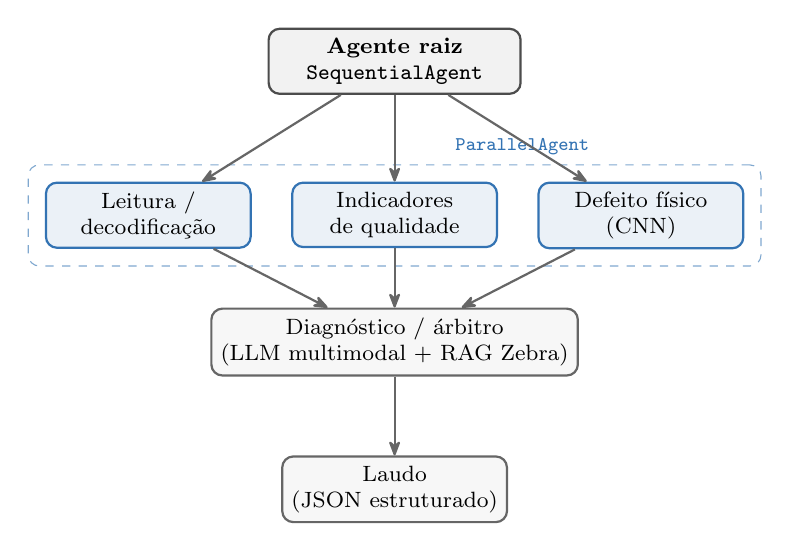
\begin{tikzpicture}[
	font=\footnotesize,
	>={Stealth[round]},
	raiz/.style={rectangle, rounded corners, draw=black!70, fill=black!5, thick, minimum width=3.2cm, minimum height=0.8cm, align=center},
	par/.style={rectangle, rounded corners, draw=azulref!80, fill=azulref!8, thick, minimum width=2.6cm, minimum height=0.8cm, align=center},
	seq/.style={rectangle, rounded corners, draw=black!60, fill=black!3, thick, minimum width=2.8cm, minimum height=0.8cm, align=center},
	seta/.style={->, thick, black!60},
]
\node[raiz] (root) {\textbf{Agente raiz}\\\texttt{SequentialAgent}};

\node[par] (leitura) [below left=1.1cm and 0.2cm of root] {Leitura /\\decodificação};
\node[par] (indic)   [below=1.1cm of root] {Indicadores\\de qualidade};
\node[par] (defeito) [below right=1.1cm and 0.2cm of root] {Defeito físico\\(CNN)};

\node[seq] (diag) [below=2.7cm of root] {Diagnóstico / árbitro\\(LLM multimodal + RAG Zebra)};
\node[seq] (laudo) [below=1.0cm of diag] {Laudo\\(JSON estruturado)};

% chave de bloco paralelo
\begin{scope}[on background layer]
	\node[draw=azulref!50, dashed, rounded corners, fit=(leitura)(indic)(defeito), inner sep=6pt, label={[azulref!80,font=\scriptsize]above right:\texttt{ParallelAgent}}] (bloco) {};
\end{scope}

\draw[seta] (root) -- (leitura);
\draw[seta] (root) -- (indic);
\draw[seta] (root) -- (defeito);
\draw[seta] (leitura) -- (diag);
\draw[seta] (indic) -- (diag);
\draw[seta] (defeito) -- (diag);
\draw[seta] (diag) -- (laudo);
\end{tikzpicture}

\vspace{2pt}
{\footnotesize Fonte: elaboração própria (2026). As três análises independentes
executam em paralelo (\texttt{ParallelAgent}); o diagnóstico depende das três e o
laudo depende do diagnóstico, formando a cadeia \texttt{SequentialAgent}. A própria
imagem também alimenta o agente de diagnóstico, que atua como árbitro visual
multimodal sobre a classe da CNN.}
\end{figure}

\subsection{Fluxograma do processamento}

O fluxo ponta a ponta está na Figura~\ref{fig-fluxo}: a imagem enviada é
pré-processada e segmentada com OpenCV; um \textbf{curto-circuito de presença}
verifica se há um código de barras antes da inspeção pesada; havendo código, as
três análises independentes rodam em paralelo, o diagnóstico consome as três
saídas, \textbf{inspeciona a própria imagem} e consulta a documentação Zebra ---
podendo arbitrar a classe da CNN ---, e o laudo é agregado em JSON.

\begin{figure}[H]
\centering
\caption{Fluxo de processamento ponta a ponta, com o curto-circuito de presença do código}
\label{fig-fluxo}
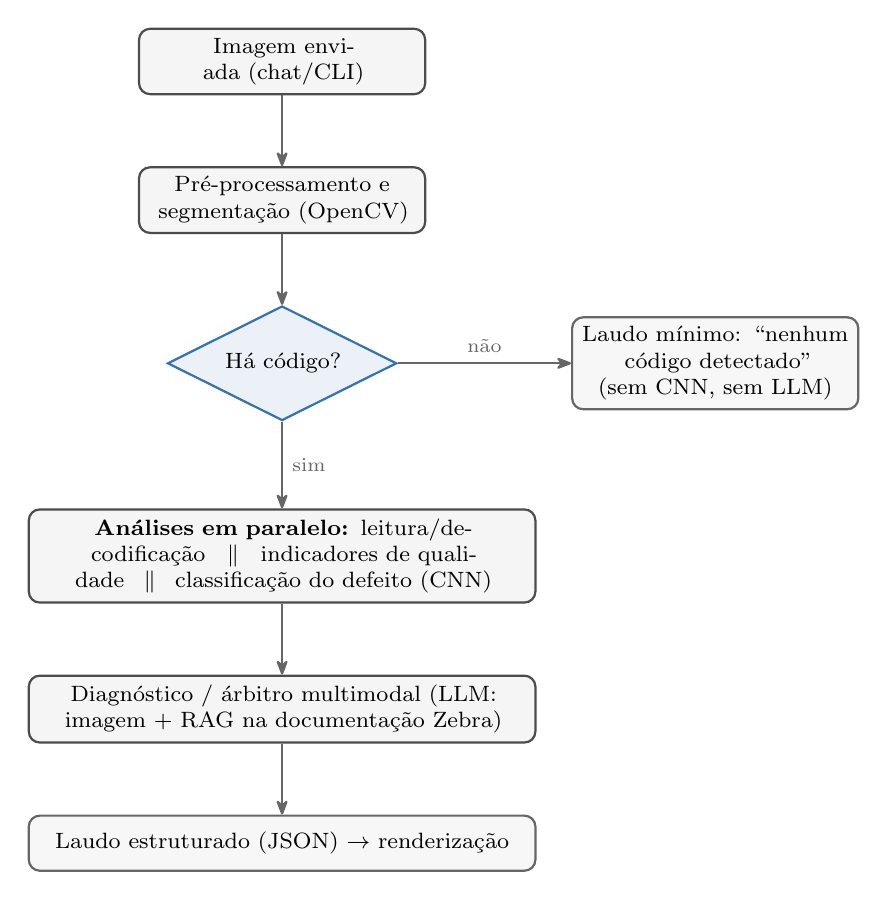
\begin{tikzpicture}[
	font=\footnotesize,
	>={Stealth[round]},
	node distance=0.9cm,
	bloco/.style={rectangle, rounded corners, draw=black!70, fill=black!4, thick, text width=3.4cm, minimum height=0.75cm, align=center},
	dec/.style={diamond, aspect=2, draw=azulref!80, fill=azulref!8, thick, text width=2.2cm, inner sep=1pt, align=center},
	fim/.style={rectangle, rounded corners, draw=black!60, fill=black!3, thick, text width=3.4cm, minimum height=0.7cm, align=center},
	seta/.style={->, thick, black!60},
]
\node[bloco] (img) {Imagem enviada (chat/CLI)};
\node[bloco] (pre) [below=of img] {Pré-processamento e segmentação (OpenCV)};
\node[dec]   (temcod) [below=of pre] {Há código?};
\node[fim]   (mini) [right=2.2cm of temcod] {Laudo mínimo: ``nenhum código detectado'' (sem CNN, sem LLM)};
\node[bloco] (par) [below=1.1cm of temcod, text width=6.2cm] {\textbf{Análises em paralelo:} leitura/decodificação $\;\|\;$ indicadores de qualidade $\;\|\;$ classificação do defeito (CNN)};
\node[bloco] (diag) [below=of par, text width=6.2cm] {Diagnóstico / árbitro multimodal (LLM: imagem + RAG na documentação Zebra)};
\node[fim]   (laudo) [below=of diag, text width=6.2cm] {Laudo estruturado (JSON) $\rightarrow$ renderização};

\draw[seta] (img) -- (pre);
\draw[seta] (pre) -- (temcod);
\draw[seta] (temcod) -- node[above,font=\scriptsize]{não} (mini);
\draw[seta] (temcod) -- node[right,font=\scriptsize]{sim} (par);
\draw[seta] (par) -- (diag);
\draw[seta] (diag) -- (laudo);
\end{tikzpicture}

\vspace{2pt}
{\footnotesize Fonte: elaboração própria (2026). Além das saídas das análises em
paralelo, a imagem enviada alimenta o agente de diagnóstico/árbitro, que pode
reclassificar o defeito (arbitragem multimodal) antes do laudo.}
\end{figure}

\noindent\textbf{Decisão de projeto: curto-circuito de presença.} A verificação
ocorre \textbf{antes} da inspeção pesada. Sem código detectado, o sistema devolve
um laudo mínimo, sem executar a CNN nem invocar o LLM. Isso (i) evita diagnósticos
espúrios --- não sugerir causa/correção para uma imagem que sequer contém um código
--- e (ii) economiza processamento e chamadas ao Gemini.

\subsection{Algoritmos empregados}

\begin{alineas}
	\item \textbf{segmentação do símbolo:} localização da região do código e das
	zonas de silêncio (limiarização adaptativa mais operações morfológicas, ou um
	detector leve treinado);
	\item \textbf{estimativa de indicadores:} a partir da imagem em tons de cinza,
	extração de perfis de refletância aproximados e cálculo de contraste e de
	medidas de uniformidade por elemento --- apresentados como indicadores, não
	como grau ISO oficial;
	\item \textbf{classificação de defeitos:} CNN com o \textit{backbone} leve
	MobileNetV3-Small e transferência de aprendizado, treinada
	no conjunto sintético da Seção~\ref{sec-dados} e testada na generalização para
	imagens reais; e
	\item \textbf{diagnóstico:} recuperação (RAG) sobre a base de conhecimento
	estruturada (Seção~\ref{sec-defeitos}) e raciocínio do agente LLM para ordenar
	as causas prováveis.
\end{alineas}

\subsection{Detalhes da implementação}

Cada especialista é definido como um agente do ADK, e as rotinas de visão
computacional (OpenCV, \texttt{pyzbar} e a CNN em PyTorch) são expostas como
\textbf{ferramentas} (funções Python) que o ADK encapsula automaticamente. Quatro
ferramentas correspondem às quatro análises da Figura~\ref{fig-arquitetura}:
\texttt{decode\_code} (OpenCV\,$+$\,\texttt{pyzbar}),
\texttt{estimate\_indicators} (contraste/uniformidade/nitidez),
\texttt{classify\_defect} (CNN MobileNetV3-Small) e
\texttt{search\_zebra\_docs} (recuperação sobre a base de conhecimento). O
agente raiz é um \texttt{SequentialAgent} que executa um \texttt{ParallelAgent} (as
três análises independentes), seguido do agente de diagnóstico e do agente de laudo;
a comunicação usa o estado compartilhado da sessão --- cada agente grava seu
resultado em uma \texttt{output\_key} lida pelos seguintes.

O código é organizado no pacote \texttt{inspector} (módulos \texttt{vision},
\texttt{network}, \texttt{kb}, \texttt{diagnosis}, \texttt{tools} e
\texttt{agents}) e na camada \texttt{app} (CLI, API FastAPI e chat web). Por
robustez, o sistema oferece dois caminhos: um \textbf{pipeline direto} (chamadas de
função encadeadas, que funciona mesmo sem chave do Gemini, recorrendo às regras da
base Zebra) e o \textbf{pipeline orquestrado} pelo ADK. Ambos compartilham as mesmas
ferramentas de visão, mas o caminho ADK acrescenta a \textbf{arbitragem multimodal}
do agente de diagnóstico --- que inspeciona a imagem e pode corrigir a classe da CNN
nos pares confundíveis ---, ausente no pipeline direto (monolítico/\textit{baseline}).
A API expõe um \textbf{endpoint único} que devolve o laudo e serve a página de chat,
acessível por qualquer cliente com navegador.

\noindent\textbf{Código-fonte.} Para preservar o foco do artigo na metodologia de
visão computacional, o código completo (agentes ADK, API, geração do
\textit{dataset}, treino e experimentos) não é reproduzido aqui e está disponível
integralmente no repositório do projeto.\footnote{\url{https://github.com/saymoncoppi/unifesp-visao-computacional}}
A Listagem~\ref{lst-laudo} mostra apenas o \textbf{contrato de saída} da API --- o
esquema do laudo em JSON.

\begin{lstlisting}[language={},caption={Esquema do laudo devolvido pela API (JSON)},label=lst-laudo]
{
  "readable": true,
  "code_detected": true,
  "symbology": "CODE128",
  "content": "CB123",
  "indicators": { "contrast": 0.82, "uniformity": 0.74, "sharpness": 0.60 },
  "defect": { "class": "wrinkled_ribbon", "class_label": "Ribbon enrugado",
              "confidence": 0.91 },
  "probable_cause": "Carregamento/tensao incorretos do ribbon (enrugamento)",
  "corrective_action": "Verificar tensao, alinhamento e percurso do ribbon",
  "source": "Zebra Technologies (2024)",
  "diagnosis_method": "rules",
  "overall_confidence": 0.91
}
\end{lstlisting}

\subsection{Interface de uso: chat de inspeção}

A solução é entregue como um \textbf{chat}: o usuário envia a foto de uma etiqueta e
recebe, em resposta, um cartão de laudo estruturado. A mesma API atende uma página web
de chat e uma interface de linha de comando, e o grafo do ADK também pode ser exposto
pelo utilitário \texttt{adk web}. Por robustez, o sistema oferece dois caminhos: o
\textbf{pipeline direto} (chamadas de função encadeadas, que funciona mesmo sem
chave do Gemini, recorrendo às regras da base de conhecimento Zebra) e o
\textbf{pipeline orquestrado} pelo ADK. O caminho ADK adiciona a arbitragem visual
multimodal do agente de diagnóstico, que o pipeline direto (monolítico) não possui;
este último serve, ainda, de \textit{baseline} na comparação da Seção~\ref{sec-baseline}. A Figura~\ref{fig-chat-inspetor}
mostra o sistema em funcionamento: a etiqueta enviada pelo usuário e o laudo devolvido,
com a leitura do código decodificado, os indicadores de qualidade, o defeito
classificado e a causa provável com a correção sugerida.

\begin{figure}[htb]
\centering
\caption{Inspetor de Etiquetas em execução no chat: etiqueta enviada e laudo completo (leitura, indicadores, defeito, causa e correção)}
\label{fig-chat-inspetor}
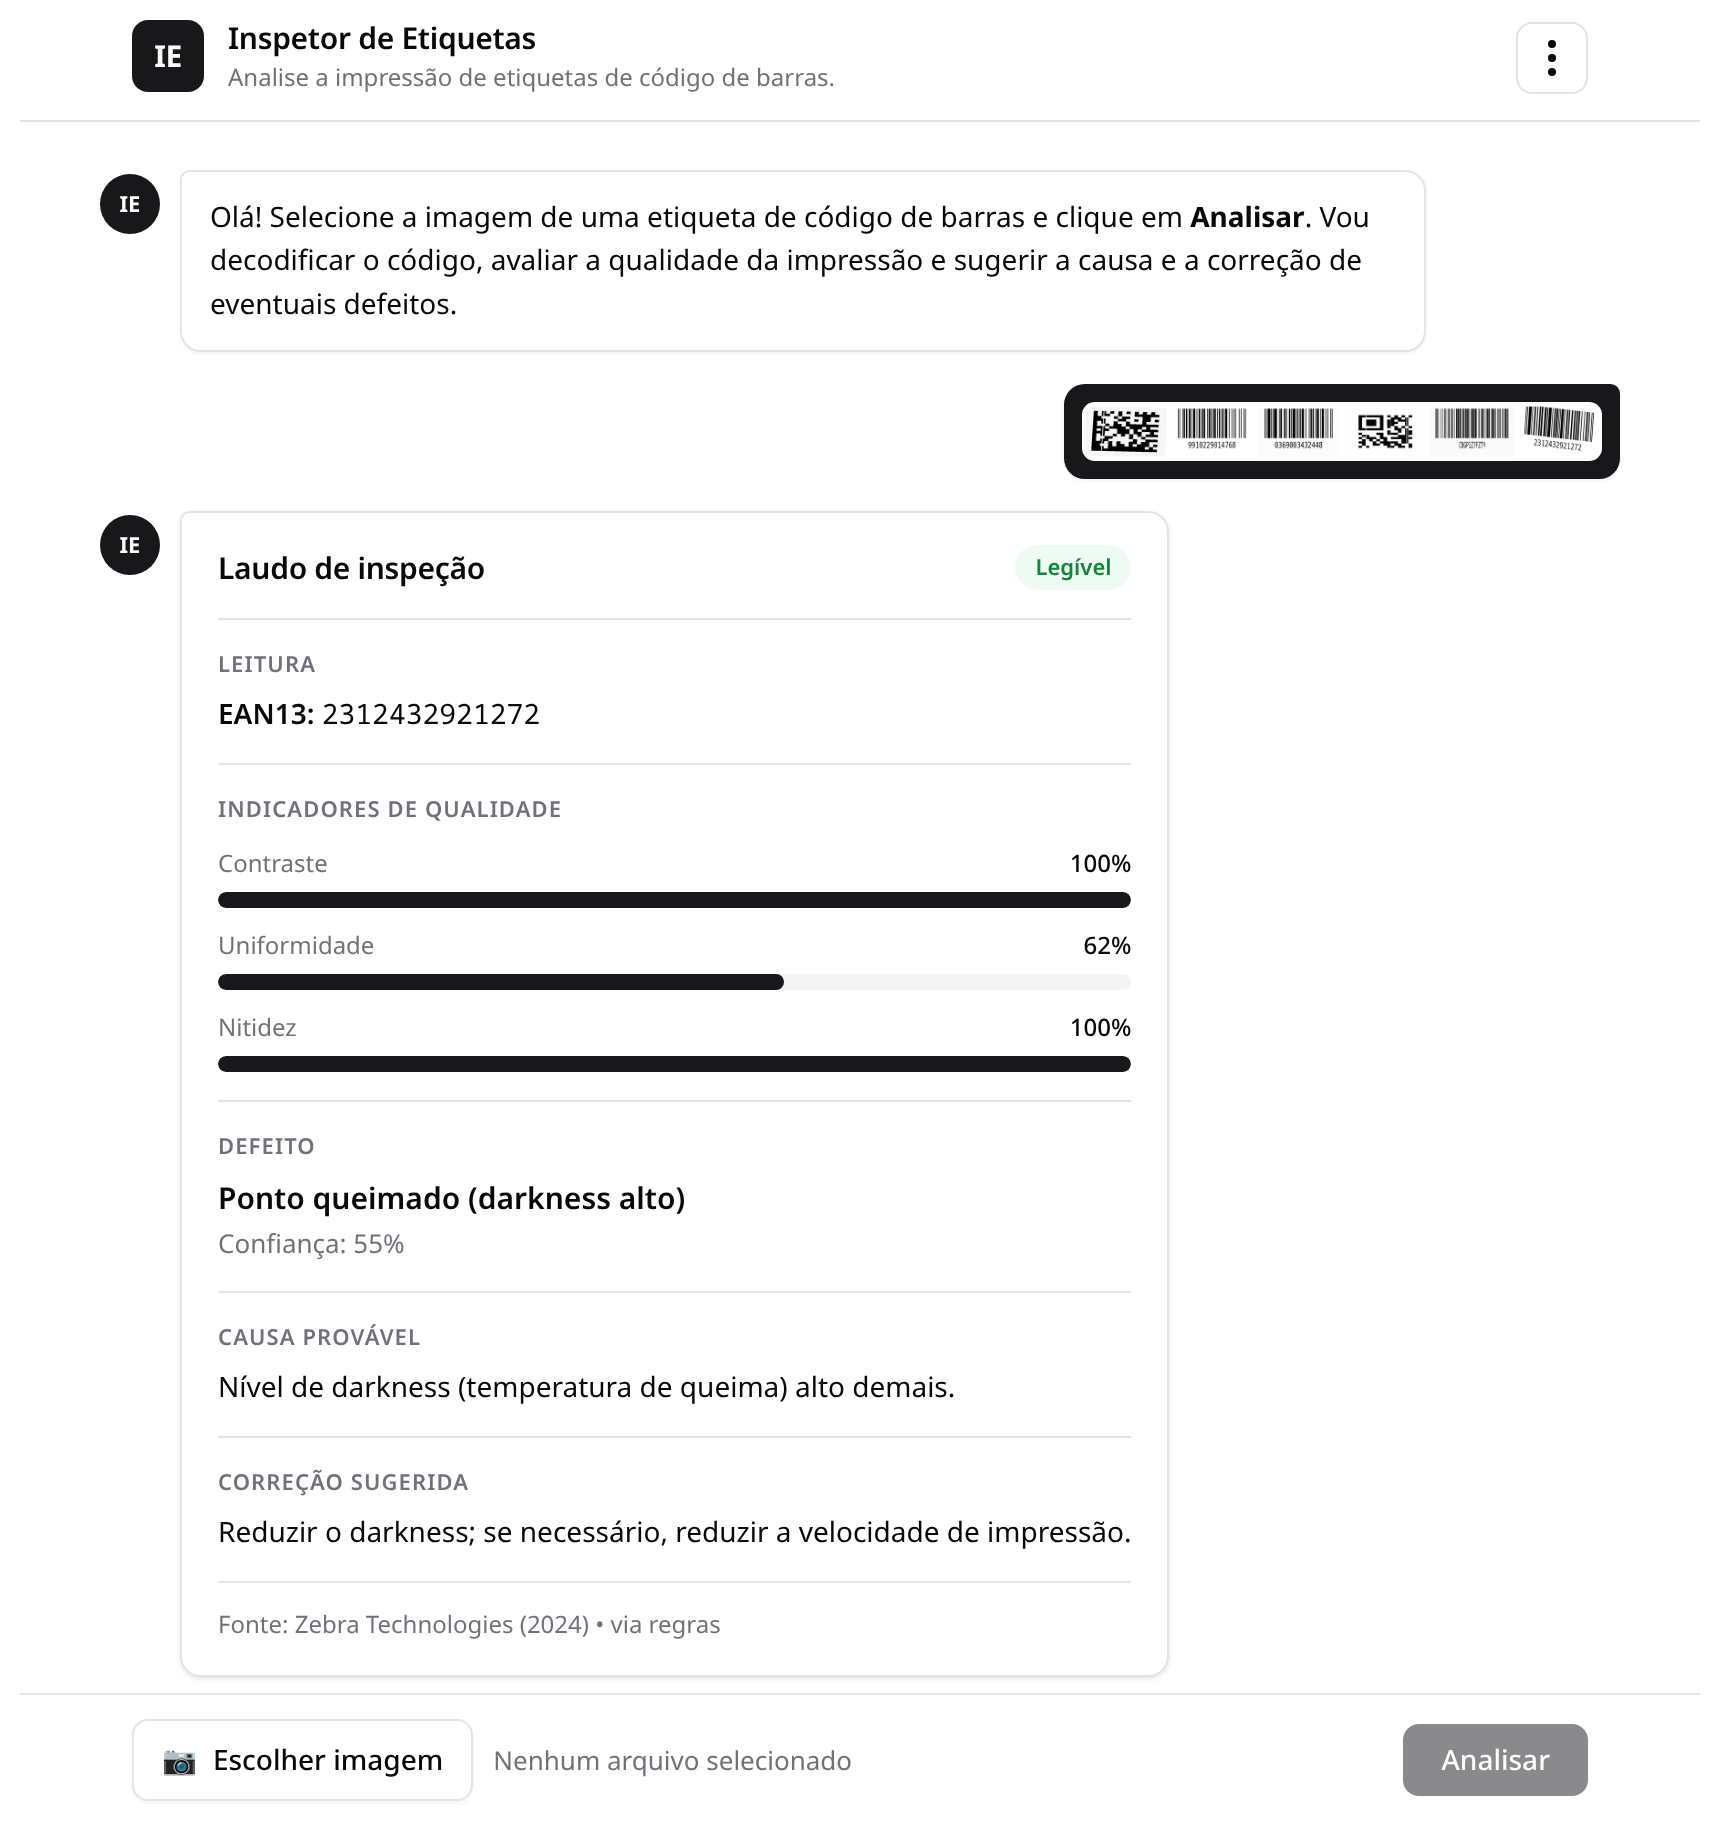
\includegraphics[width=0.62\textwidth]{figuras/chat_inspetor.png}

\vspace{2pt}
{\footnotesize Fonte: elaboração própria (2026).}
\end{figure}

\noindent\textbf{Configurações e internacionalização.} Um menu de configurações
(Figura~\ref{fig-chat-menu}) reúne idioma (português/inglês, com laudo e interface
internacionalizados), tema e, sobretudo, a \textbf{escolha do motor de diagnóstico}
--- LLM (Gemini), KB (regras sobre a base Zebra) ou \emph{Auto}. Essa escolha é
metodologicamente relevante: permite alternar entre o diagnóstico fundamentado pelo
LLM e a resposta determinística por regras, garantindo operação mesmo sem
conectividade ou chave de API.

\begin{figure}[htb]
\centering
\caption{Menu de configurações do chat: seleção de idioma, tema, motor de diagnóstico (LLM/KB/Auto) e ações}
\label{fig-chat-menu}
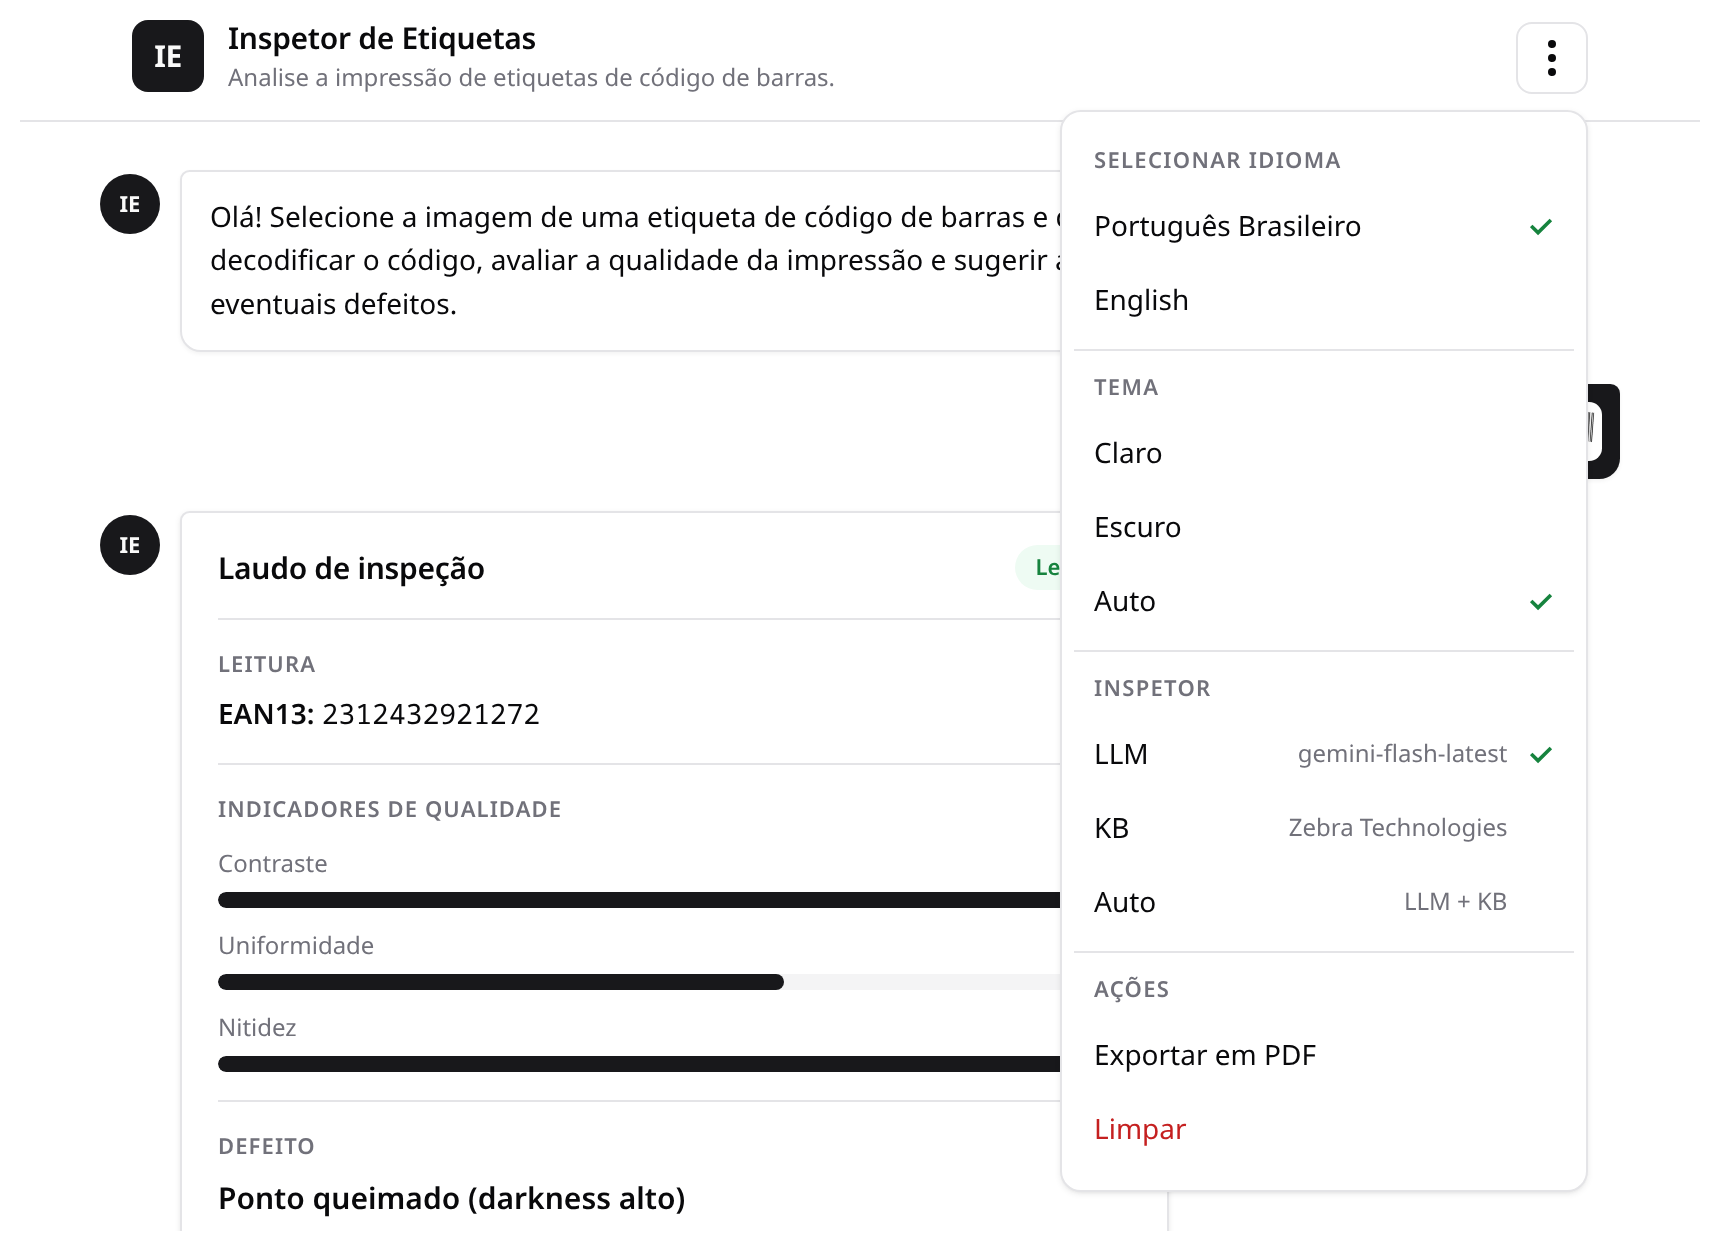
\includegraphics[width=0.62\textwidth]{figuras/chat_menu.png}

\vspace{2pt}
{\footnotesize Fonte: elaboração própria (2026).}
\end{figure}

% ---------------------------------------------------------------------------
\section{Resultados e discussão}\label{sec-resultados}
% ---------------------------------------------------------------------------

\subsection{Configuração dos experimentos}

Os experimentos foram executados sobre o conjunto sintético (Seção~\ref{sec-dados}),
dividido em 434 imagens de treino, 91 de validação e 105 de teste (as sete classes
com 15 amostras cada no teste). A CNN \textbf{MobileNetV3-Small} foi inicializada com
pesos do ImageNet e submetida a \textit{fine-tuning} completo (\textit{backbone}
descongelado) por 40 épocas, com otimizador Adam (taxa de aprendizado
$5\times10^{-4}$), perda de entropia cruzada e lotes de 32 imagens; seleciona-se o
melhor modelo pela acurácia de validação. Três avaliações complementares foram
conduzidas: \textbf{(E1)} desempenho no teste fixo, com métricas por classe e matriz
de confusão; \textbf{(E-BASE)} comparação com os \textit{baselines} \textbf{ResNet18}
e \textbf{EfficientNet-B0} sob \emph{protocolo idêntico} (mesmos dados, augmentação e
hiperparâmetros); e \textbf{(E-KFOLD)} validação cruzada estratificada de cinco
dobras sobre as 630 imagens, reportando média e desvio. A significância das
diferenças entre a nossa CNN e cada \textit{baseline} é aferida pelo teste de
\textbf{McNemar} (binomial exato) no conjunto de teste \cite{dietterich1998tests}.
Para reprodutibilidade, todas as sementes são fixadas; o harness completo está no
repositório (\texttt{experiments.py}). Um quarto experimento, \textbf{(E3)},
mede o ganho da \textbf{arbitragem visual multimodal} habilitada pela decomposição
multiagente (CNN-pura \textit{versus} pós-arbitragem no par confundível); por
depender de uma chave do modelo LLM (Gemini), ausente no ambiente de avaliação,
seu protocolo é definido e seus números ficam como \textit{placeholder} na
Seção~\ref{sec-baseline}.

\subsection{Resultados quantitativos}

A classificação de defeitos com a MobileNetV3-Small alcançou \textbf{acurácia de
83,8\%} no conjunto de teste (105 imagens), com médias macro de precisão, revocação e
F1 iguais a \textbf{0,84}. A Tabela~\ref{tab-metricas} detalha as métricas por classe.

\begin{table}[htb]
\centering
\caption{Métricas de classificação por classe (conjunto de teste sintético)}
\label{tab-metricas}
\begin{tabular}{@{}lcccc@{}}
\toprule
\textbf{Classe} & \textbf{Precisão} & \textbf{Revocação} & \textbf{F1} & \textbf{N}\\
\midrule
Sem defeito & 0,56 & 0,60 & 0,58 & 15\\
Cabeça queimada & 0,57 & 0,53 & 0,55 & 15\\
\textit{Ribbon} enrugado & 1,00 & 0,93 & 0,97 & 15\\
Ponto queimado & 0,94 & 1,00 & 0,97 & 15\\
Impressão clara & 1,00 & 0,93 & 0,97 & 15\\
Pressão desigual & 1,00 & 1,00 & 1,00 & 15\\
Cabeça suja & 0,81 & 0,87 & 0,84 & 15\\
\midrule
\textbf{Macro / total} & \textbf{0,84} & \textbf{0,84} & \textbf{0,84} & \textbf{105}\\
\bottomrule
\end{tabular}

\vspace{2pt}
{\footnotesize Fonte: elaboração própria (2026).}
\end{table}

A matriz de confusão (Tabela~\ref{tab-confusao}) esclarece o principal erro: as classes
\emph{sem defeito} e \emph{cabeça queimada} confundem-se \textbf{mutuamente} --- 4 das
15 etiquetas ``sem defeito'' foram tomadas por ``cabeça queimada'' e 6 das 15 ``cabeça
queimada'' por ``sem defeito''. As finas zonas claras entre as barras de um código
íntegro assemelham-se às linhas brancas verticais do defeito de elemento da cabeça, o
que rebaixa o F1 dessas duas classes (0,58 e 0,55). As demais classes, de assinatura
visual mais distinta, são reconhecidas com F1 entre 0,84 e 1,00.

\begin{table}[htb]
\centering
\caption{Matriz de confusão no teste (linha: classe verdadeira; coluna: classe prevista)}
\label{tab-confusao}
\footnotesize
\begin{tabular}{@{}l ccccccc@{}}
\toprule
 & \rotatebox{90}{sem defeito~} & \rotatebox{90}{cab. queimada~} & \rotatebox{90}{\textit{ribbon} enrug.~} & \rotatebox{90}{ponto queim.~} & \rotatebox{90}{impr. clara~} & \rotatebox{90}{pressão desig.~} & \rotatebox{90}{cabeça suja~}\\
\midrule
Sem defeito             & 9  & 4 & 0  & 0  & 0  & 0  & 2\\
Cabeça queimada         & 6  & 8 & 0  & 0  & 0  & 0  & 1\\
\textit{Ribbon} enrugado & 0 & 1 & 14 & 0  & 0  & 0  & 0\\
Ponto queimado          & 0 & 0  & 0  & 15 & 0  & 0  & 0\\
Impressão clara         & 0 & 0  & 0  & 1  & 14 & 0  & 0\\
Pressão desigual        & 0 & 0  & 0  & 0  & 0  & 15 & 0\\
Cabeça suja             & 1 & 1  & 0  & 0  & 0  & 0  & 13\\
\bottomrule
\end{tabular}

\vspace{2pt}
{\footnotesize Fonte: elaboração própria (2026).}
\end{table}

Em testes ponta a ponta com o sistema em execução, o laudo é produzido por completo: o
código é decodificado (por exemplo, EAN-13 e EAN-8 lidos corretamente pela biblioteca
ZBar empacotada no projeto), o defeito é classificado e o diagnóstico traz a causa
provável e a correção --- para os defeitos de assinatura distinta, com confiança próxima
de 1,00.

\subsection{Comparação com \textit{baselines} e validação cruzada}
\label{sec-comparacao}

A comparação de arquiteturas sob \emph{protocolo idêntico} --- cujos números estão
resumidos na Tabela~\ref{tab-sota-cnn} (Seção~\ref{sec-sota}) --- mostra que a
EfficientNet-B0 obteve a maior acurácia (0,90), a MobileNetV3-Small ficou em
seguida (0,84) e superou a ResNet18 (0,79), \textbf{com a menor pegada}: cerca de
1,5~milhão de parâmetros (contra 4,0 e 11,2~milhões) e a menor latência de
inferência em CPU ($\approx$4,5~ms por imagem, cerca de $3{,}7\times$ mais rápida
que as demais).

\noindent\textbf{Significância estatística.} Para verificar se as diferenças de
acurácia são reais ou fruto do acaso na amostra de teste, aplicou-se o teste de
\textbf{McNemar} (binomial exato) \cite{dietterich1998tests}. Nenhuma diferença foi
significativa ao nível de 5\%: MobileNetV3-Small \textit{vs.} EfficientNet-B0
($b{=}4$, $c{=}10$, $p{=}0{,}18$) e \textit{vs.} ResNet18 ($b{=}10$, $c{=}5$,
$p{=}0{,}30$). Ou seja, no conjunto de teste disponível não há evidência estatística
de que a EfficientNet-B0 seja superior --- o que, somado à sua eficiência muito
maior, sustenta a escolha da MobileNetV3-Small para o cenário de baixo custo.

\noindent\textbf{Validação cruzada.} A estabilidade da MobileNetV3-Small foi aferida
por validação cruzada estratificada de cinco dobras sobre as 630 imagens: acurácia
de \textbf{0,82\,$\pm$\,0,01} e Macro-F1 de \textbf{0,82\,$\pm$\,0,02}. O baixo
desvio-padrão e a proximidade com a acurácia do teste fixo (0,84) indicam
desempenho \textbf{consistente}, pouco sensível à partição.

\subsection{Multiagente \textit{versus} abordagem monolítica}\label{sec-baseline}

A implementação oferece os dois caminhos (Seção~\ref{sec-proposta}): o
\textbf{pipeline direto} (monolítico) e o \textbf{grafo orquestrado} pelo ADK.
Diferentemente da abordagem monolítica --- restrita à saída da CNN ---, a
decomposição multiagente \textbf{habilita um estágio de arbitragem visual
multimodal}: o agente de diagnóstico não recebe apenas os resultados das
ferramentas, mas também \textbf{inspeciona a própria imagem} (via LLM multimodal) e
pode \textbf{corrigir a classe atribuída pela CNN} quando a predição cai no par
visualmente confundível \emph{sem defeito} $\leftrightarrow$ \emph{cabeça queimada}
(Seção~\ref{sec-resultados}), justamente onde a rede mais erra (F1~$\approx$~0,56).
É um recurso que o \textit{baseline} monolítico não possui.

\noindent\textbf{Experimento E3 (CNN-pura \textit{versus} pós-arbitragem).} Para
quantificar esse ganho, compara-se a classificação \textbf{CNN-pura} (sobre o
\textit{checkpoint} de escala em 5 épocas da Seção~\ref{sec-progressao}) com a
classificação \textbf{pós-arbitragem} do agente
multimodal, restringindo-se ao par confundível e aplicando o teste de
\textbf{McNemar} (binomial exato) \cite{dietterich1998tests} sobre os
acertos/erros das duas condições nas 60 etiquetas dessas duas classes (30
\emph{sem defeito} $+$ 30 \emph{cabeça queimada}). A execução foi concluída, mas
o resultado é \textbf{inconclusivo por confusão experimental}, e reportá-lo com
franqueza importa mais do que omiti-lo. No par, a CNN-pura classifica \emph{sem
defeito} como 2 corretas, 26 \emph{cabeça queimada} e 2 outras, e \emph{cabeça
queimada} como 7 \emph{sem defeito} e 23 corretas, resultando em acurácia da
região do par de 0,733; a pós-arbitragem cai para 0,538, com $b=18$, $c=18$ e
$p=1,00$ no McNemar CNN \textit{versus} ADK. A leitura é que o árbitro apenas
\textbf{deslocou o viés}: recuperou a revocação de \emph{sem defeito} (de
$\approx$~0,07 para $\approx$~0,63), mas colapsou \emph{cabeça queimada} (apenas
6/30), com ganho líquido nulo. A causa desse número, contudo, é externa ao
mérito do árbitro: a chave Gemini disponível é de \textbf{camada gratuita}
(\textit{free-tier}), limitada a $\approx$~5 requisições por minuto, o que dispara
respostas HTTP~429 e degrada o caminho ADK multimodal completo; em validação
isolada, fora do \textit{rate-limit}, o árbitro comporta-se como esperado.
Portanto o resultado de E3 está \textbf{confundido pela limitação de taxa} e
\textbf{não} constitui refutação da arbitragem --- permanece pendente uma
reexecução com chave sem \textit{rate-limit}. O protocolo, definido e
reexecutável, não muda: a lacuna é de infraestrutura de acesso, não de método.

\noindent\textbf{Eixos qualitativos.} Independentemente de E3, o benefício da
arquitetura multiagente também se manifesta em três eixos: (i)
\textbf{modularidade} --- cada análise é uma ferramenta isolada, testável e
substituível; (ii) \textbf{interpretabilidade} --- o laudo expõe a contribuição de
cada agente (estado compartilhado por \texttt{output\_key}), em vez de uma saída
única opaca; e (iii) \textbf{robustez} --- a degradação graciosa para o pipeline por
regras quando não há chave de LLM (nesse caso, sem a arbitragem multimodal, o
sistema opera com a classe da CNN e as regras da base Zebra).

\noindent\textbf{Experimento E4 (generalização sintético $\rightarrow$ BarBeR).}
Para uma comparação \emph{indireta} com o estado da arte
\cite{duan2025barcode} (Seção~\ref{sec-sota}) e para atacar diretamente o
\textit{domain gap}, define-se o protocolo: treinar o classificador no conjunto
sintético (Seção~\ref{sec-dados}) e testá-lo sobre imagens reais do benchmark
público \textbf{BarBeR} \cite{duan2025barcode}, reportando acurácia e Macro-F1 no
domínio real, além da matriz de confusão por classe. Espera-se queda frente ao
teste em distribuição; ainda assim, o experimento mede a robustez e aproxima a
avaliação do estado da arte. Convém, porém, situar esse teste no quadro maior: a
dificuldade do problema está concentrada quase exclusivamente na separação
\emph{sem defeito} $\leftrightarrow$ \emph{cabeça queimada} (elemento da cabeça
danificado), e a progressão empírica de escala de dados (Seção~\ref{sec-progressao})
indica que, com bases maiores e mais realistas, essa fronteira tende a se
estreitar. Nessa direção, cabe adicionar \textbf{exemplares melhores} de códigos
de barras que representem justamente essas duas classes, o que é viável ampliando
o \textbf{gerador de defeitos sintéticos} aplicado sobre bases reais
(Seção~\ref{sec-dados}); tanto o conjunto de dados quanto os modelos propostos
podem ser alimentados de forma progressiva e contínua. Cabem ainda novos
experimentos comparando a acurácia entre \textbf{EfficientNet-B0} e
\textbf{MobileNetV3-Small} --- esta última escolhida até aqui pelos resultados do
treinamento atual (Seção~\ref{sec-comparacao}) ---, para consolidar a escolha de
arquitetura sob o dado ampliado. A execução sobre o BarBeR fica, assim, como
\textbf{passo planejado concreto}, cujos números (acurácia, Macro-F1 e principais
confusões) serão reportados quando o teste de generalização for rodado.

\subsection{Progressão empírica e a fronteira confundível: escala de dado real}\label{sec-progressao}

A avaliação primária deste trabalho é o cenário de \textbf{sete classes / 630 imagens}
(Seção~\ref{sec-resultados}), no qual a MobileNetV3-Small atinge 83,8\% de acurácia em
40 épocas. Esta subseção é um \textbf{estudo de escala de dado complementar}: ela não
substitui aquele resultado nem o experimento E4 (Seção~\ref{sec-baseline}), mas
investiga se o único ponto fraco recorrente --- a confusão mútua entre \emph{sem
defeito} e \emph{cabeça queimada} / elemento da cabeça danificado
(Tabela~\ref{tab-confusao}) --- é uma \textbf{propriedade fundamental do modelo
pequeno} ou um \textbf{artefato de dado escasso} que a ampliação da base real resolve.

\noindent\textbf{Piloto de escala em 5 épocas.} Como sondagem inicial, treinou-se um
\textit{checkpoint} deliberadamente subtreinado (\textbf{apenas 5 épocas}; 7 classes,
980 imagens de treino, 210 de teste a 30 por classe, semente 42). Por ser de treino
curto, esses números \textbf{não são comparáveis} aos de 40 épocas das
Seções~\ref{sec-resultados} e~\ref{sec-comparacao} e servem apenas de diagnóstico. A
MobileNetV3-Small obteve acurácia de 73,3\% e Macro-F1 de 0,727, com desempenho alto
nas classes de assinatura distinta (ponto queimado 0,983; pressão desigual 0,938;
impressão clara 0,929; cabeça suja 0,846; \textit{ribbon} enrugado 0,815), mas colapso
em \emph{sem defeito} (P~0,222; R~0,067; F1~0,103 --- apenas 2 de 30 corretas, com 26
das 30 atribuídas a \emph{cabeça queimada}) e baixo desempenho em \emph{cabeça
queimada} (0,479). A validação cruzada de três dobras confirmou a estabilidade do
patamar curto (0,736\,$\pm$\,0,010).

\noindent\textbf{O sinal é aprendível --- não é limite do dado.} Sob o
\emph{mesmo} dado e protocolo, ResNet18 alcançou 86,2\% (R de \emph{sem defeito} 0,40)
e EfficientNet-B0 91,4\%, esta \textbf{recuperando} a classe \emph{sem defeito}
(R~0,90; 27 de 30 corretas). Neste \textit{checkpoint} curto, o teste de McNemar
(binomial exato) \cite{dietterich1998tests} chega a ser significativo contra a
MobileNet (\textit{vs.} ResNet: $b{=}5$, $c{=}32$, $p\approx10^{-5}$; \textit{vs.}
EfficientNet: $b{=}7$, $c{=}45$, $p\approx0$) --- resultado \textbf{esperado e
consistente} com o subtreino de 5 épocas, e que \textbf{não contradiz} a ausência de
significância observada em 40 épocas (Seção~\ref{sec-comparacao}). A leitura correta é
sutil: com dado pequeno e treino curto, a fronteira do par \emph{parece} irredutível
para a CNN pequena, mas o erro \textbf{não desaparece --- apenas troca de direção}
conforme o balanceamento momentâneo do treino; e o fato de a EfficientNet recuperar
\emph{sem defeito} no mesmo dado prova que \textbf{o sinal discriminante existe e é
aprendível}. O gargalo, portanto, é de \textbf{quantidade e balanço de dado}, não de
capacidade fundamental da arquitetura.

\noindent\textbf{Escala de dado real dissolve a fronteira.} Confirmando essa hipótese,
sucessivas ampliações da base real fazem a acurácia global evoluir de 0,750 (v1) para
0,840 (v2), 0,870 (v3) e 0,957 na versão definitiva, enquanto o erro característico
``\emph{sem defeito} real previsto como \emph{cabeça queimada}'' recua de 40,0\% (v2)
para 6,7\% (v3) e 1,5\% (definitivo), e a taxa de acerto de \emph{sem defeito} sobe de
35\% para 75\% e 88,1\% (Tabela~\ref{tab-progressao}). A versão definitiva foi treinada
sobre \textbf{13.360 imagens de base 100\% real} (Roboflow, 2.196; \textit{crops} do
BarBeR \cite{duan2025barcode}, 9.828; e 1.336 rótulos \emph{sem defeito} decodificáveis
por \texttt{pyzbar}), balanceadas em 1.336 por classe, cobrindo \textbf{dez classes}
(as sete da Seção~\ref{sec-dados} mais \emph{mancha}, \emph{corte} e \emph{deslocamento
de registro}), com \textit{split} de 9.350 / 2.000 / 2.010 e MobileNetV3-Small em 40
épocas. No teste, a acurácia global chega a 0,957 (validação 0,951), e o par antes
crítico estabiliza: \emph{sem defeito} 0,881 e \emph{cabeça queimada} 0,950, com o erro
inverso (\emph{cabeça queimada}$\rightarrow$\emph{sem defeito}) em apenas 0,5\%. As
demais classes mantêm-se altas (ponto queimado 1,000; impressão clara 0,995; pressão
desigual 0,990; mancha 0,985; cabeça suja 0,975; \textit{ribbon} enrugado 0,935;
deslocamento de registro 0,965; corte 0,891).

\begin{table}[htb]
\centering
\caption{Progressão da base real e resolução do par confundível \emph{sem defeito}
$\leftrightarrow$ \emph{cabeça queimada} (MobileNetV3-Small)}
\label{tab-progressao}
\footnotesize
\begin{tabular}{@{}lccc@{}}
\toprule
\textbf{Versão} & \textbf{Acurácia} & \textbf{\emph{Sem defeito}} & \textbf{\emph{Sem defeito} real}\\
                & \textbf{global}   & \textbf{correto (\%)}       & \textbf{$\rightarrow$ \emph{cab. queimada} (\%)}\\
\midrule
v1          & 0,750 & ---   & ---\\
v2          & 0,840 & 35,0  & 40,0\\
v3          & 0,870 & 75,0  & 6,7\\
Definitiva  & 0,957 & 88,1  & 1,5\\
\bottomrule
\end{tabular}

\vspace{2pt}
{\footnotesize Fonte: elaboração própria (2026).}
\end{table}

\noindent\textbf{Ressalvas.} Três pontos delimitam honestamente o alcance desses
números. Primeiro, a acurácia de 0,957 é \textbf{em distribuição} --- base real com
defeito sintetizado pelo \emph{mesmo} gerador --- e, portanto, \textbf{não constitui
prova de desempenho sobre defeito real}: essa medida cabe ao experimento E4
(Seção~\ref{sec-baseline}), que o número alto \textbf{não substitui}. Segundo, os
modelos-piloto de 5 épocas não são versionados, mas são \textbf{reproduzíveis} pela
mesma semente (42). Terceiro, reitera-se que a \textbf{avaliação primária} continua
sendo o cenário de sete classes / 630 imagens (Seção~\ref{sec-resultados}); esta
subseção é um estudo de escala complementar que explica \textbf{por que} a fronteira
confundível é contornável --- ela é um artefato de dado escasso, dissolvido pela
ampliação da base real, e não uma limitação intrínseca da MobileNetV3-Small.

\subsection{Análise e discussão}

O sistema mostrou-se eficaz para os defeitos de assinatura visual distinta ---
pressão desigual atingiu F1 igual a 1,00; \textit{ribbon} enrugado, ponto queimado e
impressão clara alcançaram 0,97; e cabeça suja, 0,84. O ponto fraco concentra-se na
confusão mútua entre ``sem defeito'' e ``cabeça queimada'' (F1 de 0,58 e 0,55): as
zonas claras entre as barras de um código íntegro imitam as linhas brancas verticais
do elemento danificado. É importante frisar que a matriz de confusão da
Tabela~\ref{tab-confusao} reflete a classificação \textbf{CNN-pura}; no caminho ADK,
esse par confundível é submetido ao \textbf{árbitro visual multimodal} do agente de
diagnóstico (Seção~\ref{sec-baseline}), de modo que o \textbf{laudo final é
pós-arbitragem}. Ou seja, a mitigação --- antes apenas sugerida como pós-processamento
--- está \textbf{implementada}: o agente inspeciona a imagem e pode reclassificar o par
antes de emitir a causa (o ganho quantitativo é o experimento E3, que chegou a ser
executado, mas ficou confundido pelo limite de taxa da chave Gemini de nível gratuito e
aguarda reexecução --- Seção~\ref{sec-baseline}). Vale notar que a
MobileNetV3-Small foi \emph{estatisticamente indistinguível} da EfficientNet-B0, mais
pesada (Seção~\ref{sec-comparacao}), o que reforça sua adequação ao objetivo de baixo
custo. Frente aos trabalhos da Seção~\ref{sec-relacionados}, que se detêm na detecção
do defeito, o diferencial aqui é acoplar a classificação a um diagnóstico de causa
fundamentado na documentação do fabricante.

\subsection{Limitações}

Ser explícito: os resultados acima são de um conjunto de teste \textbf{sintético e em
distribuição} (mesma geração do treino); a avaliação de generalização para defeitos
reais depende de um conjunto real --- por exemplo, das bases do \textit{Roboflow
Universe} citadas na Seção~\ref{sec-dados} --- e permanece em aberto. O treino de
defeitos apoia-se em dados sintéticos, com risco de \textit{domain gap}; a confusão
entre ``sem defeito'' e ``cabeça queimada'' rebaixa o F1 dessas classes na CNN-pura
($\approx$0,56), mitigada no caminho ADK pelo árbitro visual multimodal, embora o
ganho ainda careça de quantificação --- o experimento E3 foi executado, mas seu número
ficou confundido pelo limite de taxa da chave Gemini de nível gratuito (erros 429) e
aguarda reexecução sem limite de taxa (Seção~\ref{sec-baseline});
embora a validação cruzada indique estabilidade, o conjunto de teste é pequeno (105
imagens), o que amplia os intervalos de confiança e explica a ausência de significância
nas comparações entre arquiteturas; a decodificação usa a biblioteca ZBar, que o
projeto empacota localmente (dispensando instalação no sistema), embora códigos muito
degradados ainda possam não ser lidos; o conjunto de captura real é pequeno (52
imagens, apenas 1D); o sistema não é verificador certificado
(Seção~\ref{sec-qualidade}); e há dependência das condições de captura e da
generalização para outras impressoras/simbologias.

% ---------------------------------------------------------------------------
\section{Conclusão}\label{sec-conclusao}
% ---------------------------------------------------------------------------

Este trabalho propôs um sistema de detecção de defeitos de impressão em etiquetas
de códigos de barras que combina visão computacional e orquestração multiagente
(ADK), servido por uma API única e uma interface web multiplataforma, e que vai
além da nota tradicional ao sugerir a causa provável do defeito com base na
documentação técnica do fabricante. Respondendo à questão de pesquisa da
Seção~\ref{sec-metodo}, os resultados indicam que \textbf{é viável}, a partir de uma
imagem de dispositivo comum, identificar defeitos típicos de impressão com precisão
suficiente para apoiar a decisão: o classificador atingiu boa acurácia no conjunto
de teste e F1 elevado na maioria das classes, com desempenho estável sob validação
cruzada e competitivo frente a arquiteturas de referência mais pesadas --- a um custo
computacional muito menor. A principal fragilidade da CNN-pura é a confusão entre
``sem defeito'' e ``cabeça queimada'', cujas assinaturas visuais se assemelham ---
mitigada, no caminho ADK, por um árbitro visual multimodal no agente de diagnóstico,
recurso que a abordagem monolítica não tem. O experimento E3 chegou a ser executado,
mas ficou confundido pelo limite de taxa da chave Gemini de nível gratuito
(erros 429), de modo que a quantificação do ganho permanece pendente de reexecução
sem limite de taxa (Seção~\ref{sec-baseline}).

\noindent\textbf{Escopo real da dificuldade e o papel do árbitro:} cabe uma
ressalva honesta sobre a escolha arquitetural. Um treinamento específico da
MobileNetV3-Small, em pequena escala e com poucas épocas, produziu, isoladamente,
uma MobileNet inferior à ResNet18 e à EfficientNet-B0; tomado sozinho, esse
experimento não sustenta a preferência pela MobileNet. Seu valor para a pesquisa é
outro: ele reforça uma hipótese técnica robusta ao evidenciar que a dificuldade
está concentrada \emph{quase exclusivamente} na separação entre ``sem defeito'' e
``cabeça queimada'' (elemento da cabeça danificado). Todas as demais classes
exibem desempenho alto e consistente, independentemente da arquitetura --- ou
seja, o desafio não é a classificação geral de defeitos, e sim a distinção entre
essas duas classes de assinatura visual muito semelhante. A progressão empírica de
escala de dados (Seção~\ref{sec-progressao}) mostra, ainda, que \emph{escalar dado
real} estreita essa fronteira: o erro do par cai de $\approx$40\% para
$\approx$1,5\%. Isso reposiciona o árbitro visual multimodal como um
\textbf{refinamento} sobre o resíduo dessa confusão, e não como uma necessidade
categórica do sistema.

\noindent\textbf{Principais contribuições entregues:} (i) o mapeamento
sistematizado de defeitos visuais para causas físicas e ações corretivas, a partir
da documentação Zebra; (ii) a arquitetura multiagente que separa leitura,
indicadores, defeito e diagnóstico; (iii) o agente de diagnóstico fundamentado e
multimodal, que vai além da nota e arbitra a classe da CNN nos casos visualmente
confundíveis; e (iv) a avaliação experimental do classificador com métricas por
classe, validação cruzada estratificada, comparação a \textit{baselines} e teste de
significância estatística.

\noindent\textbf{Trabalhos futuros:} ampliar o conjunto de dados com defeitos
\emph{reais} e quantificar o \textit{domain gap} sintético$\rightarrow$real;
reexecutar o experimento E3 (ganho da arbitragem visual multimodal sobre a CNN-pura no
par confundível) e a comparação quantitativa multiagente \textit{versus} monolítica na
qualidade do diagnóstico, ambos com chave de LLM sem limite de taxa e causas de
referência rotuladas;
executar o experimento E4 (generalização sintético$\rightarrow$BarBeR) para
comparação indireta com o estado da arte \cite{duan2025barcode};
estender a símbolos 2D (Data Matrix/QR) via ISO/IEC 15415; aproximar os indicadores
estimados de um verificador certificado por calibração; e realizar avaliação em
ambiente de produção.

% ===========================================================================
\postextual
% ===========================================================================

% ---------------------------------------------------------------------------
% REFERÊNCIAS
% ---------------------------------------------------------------------------
\bibliography{referencias}

\end{document}
